\documentclass[deposito, acronym, symbols]{fei}

%\usepackage{glossaries}
\usepackage{subcaption} 
\usepackage{graphicx}
\usepackage{float}
%\usepackage{units}
\usepackage[portuguese]{algorithm2e}
\usepackage{biblatex}
\usepackage{amsmath}
\usepackage{listings}
%\lstset{frame=tb,
%literate= {á}{{\'a}}1 {â}{{\^a}}1 {ã}{{\~a}}1 {é}{{\'e}}1 {ê}{\^e}1 {ç}{\c{c}}1 {í}{\i}1 {ú}{\'u}1 {ó}{{\'o}}1 {ô}{{\^o}}1 {õ}{{\~o}}1 {Á}{{\'A}}1 {É}{{\'E}}1, }
\usepackage[utf8]{inputenc}
\usepackage{chngcntr} %Faz com que o numero das notas de rodape aumente crescentemente.
\usepackage{appendix}
\counterwithout{footnote}{chapter}% "
\usepackage{siunitx}
\sisetup{output-exponent-marker=\ensuremath{\mathrm{e}}} %Escrita que precede cada entrada na lista de ilustrações.
\renewcommand{\cftfigurepresnum}{Figura }
\setlength{\cftfigurenumwidth}{5.7em}



\usepackage{titling}
\addbibresource{Referencias.bib}
%\bibliographystyle{plain}
\bibliography{Referencias}
\graphicspath{ {Imagens/}, {Tabelas/}}

\begin{document}

%CAPA
\begin{titlepage}
      \begin{center}
      \Large CENTRO UNIVERSITÁRIO FEI \\ DEPARTAMENTO DE ENGENHARIA MECÂNICA
      \vspace{3 cm}
      \Large \textbf{\\PROJETO DE FORJAMENTO}
      \end{center}

    \vspace {2 cm}
    \hfill \parbox{8 cm}{Relatório apresentado ao departamento de Engenharia Mecânica do Centro Universitário FEI, como parte dos requisitos de avaliação da disciplina MEF130 – Processos de Fabricação por Conformação Plástica. Solicitado pelo Prof. Dr.-Ing. Mauro Moraes de Souza.}
    \vspace{2 cm}

    Nomes e registros acadêmicos dos autores: (Grupo: 006) – 20/nov/2023
    \vspace{1 cm}
    \begin{center}
      1. Felipe Estevão Coquito de Mello - 11.120.486-3 \\ 2. Gabriel Mola da Silva - 11.120.255-2 \\ 3. Netuno Trindade Torrente Rovaroto - 11.120.321-2 \\ 4. Vitoria Fedatto Stefaneli - 11.120.497-0
      \vspace{3 cm}
      \\ São Bernardo do Campo \\ 2023
    \end{center}
    \thispagestyle{empty}
    \setcounter{page}{0}
\end{titlepage}

\tableofcontents
\listoffigures
\listoftables

\begin{resumo}

O processo de forjamento é muito importante, principalmente por sua escalabilidade que influencia em reduções de preço no processo de fabricação e o custo/benefício supera em muito nos processos de usinagem. Além disso, o forjamento tem algumas vantagens, como: este processo não retira material, ele somente o modela e ele pode ser combinado com processos de usinagem como o fresamento e o torneamento. Portanto o estudo dos processos de forjamento é muito importante. Este relatório teve como objetivo contemplar toda a trajetória do projeto de forjamento a quente, desde o início com o desenho da peça usinada, a criação da peça forjada, com as cotas e tolerâncias, a criação da matriz, até o final do processo com as simulações no software Simufact Forming e cálculos de esforços no forjamento. Os resultados foram favoráveis e estão dentro do esperado, concluiu-se, então, que o projeto se mostrou satisfatório e cumpre com todas as normas estabelecidas.

\palavraschave{Forjamento a quente, Simulação, Simufact Forming}

\end{resumo}

\chapter{Introdução}

Ao longo do semestre um dos alvos de estudo foi o Forjamento e sua importância para o mundo, principalmente pela possibilidade de escalabilidade que influencia na reduções do preço deste processo de fabricação que supera em muito no quesito custo/benefício de peças produzidas por processos de Usinagem.

O Forjamento pode ser definido como um processo de fabricação onde se modifica-se a geometria dos metais para peças específicas definidas pelo projetista, através de esforços compressivos. Este processo pode acontecer em diferentes faixas de temperatura sendo normalmente divididos em Forjamento a Frio e Forjamento a Quente.

As vantagens da utilização de procedimentos de Forjamento, além da escalabilidade como citado anteriormente é o fato de ser um processo que modela o material em vez de retirar, como o usinado, isso significa um menor número de desperdício de matéria prima. Outra vantagem é que está técnica pode ser combinada com outras como de Fresamento ou Torneamento, funcionando como um processo intermediário para facilitar processos seguintes.


\section{Objetivos do trabalho}

Sabendo da imensa influência que a área de Forjaria possui, principalmente seu impacto na área onde engenheiros mecânicos atuam, se vê a necessidade de elaborar um trabalho onde contemple toda a trajetória de um projeto mecânico voltado para está área, com cunho de entender como é o dia a dia desta carreira.


Será desenvolvido uma peça com as especificações fornecidas pelo professor orientador, a partir do Forjado será elaborado as Matrizes Superiores e Inferiores do projeto, assim como os cálculos das Forças, que serão necessários para a eventual Simulação do Forjamento utilizando o software \textit{Simufact Forming}. 

\chapter{Referencial teórico} \label{tabelas}

Para a realização do projeto é necessário o uso de tabelas e normas. Neste tópico serão apresentadas as tabelas e normas utilizadas durante todo o projeto.

\section{Tabelas} 

A tabelas estão apresentadas em ordem de uso.

A Tabela \ref{tab:tabA4} foi utilizada para a definição das inclinações laterais. Como a máquina escolhida foi uma prensa normal os ângulos internos e externos foram $6^\circ$ e $3^\circ$, respectivamente.

\begin{table}[!htb]
 \centering
    \caption{Tabela A/4}
    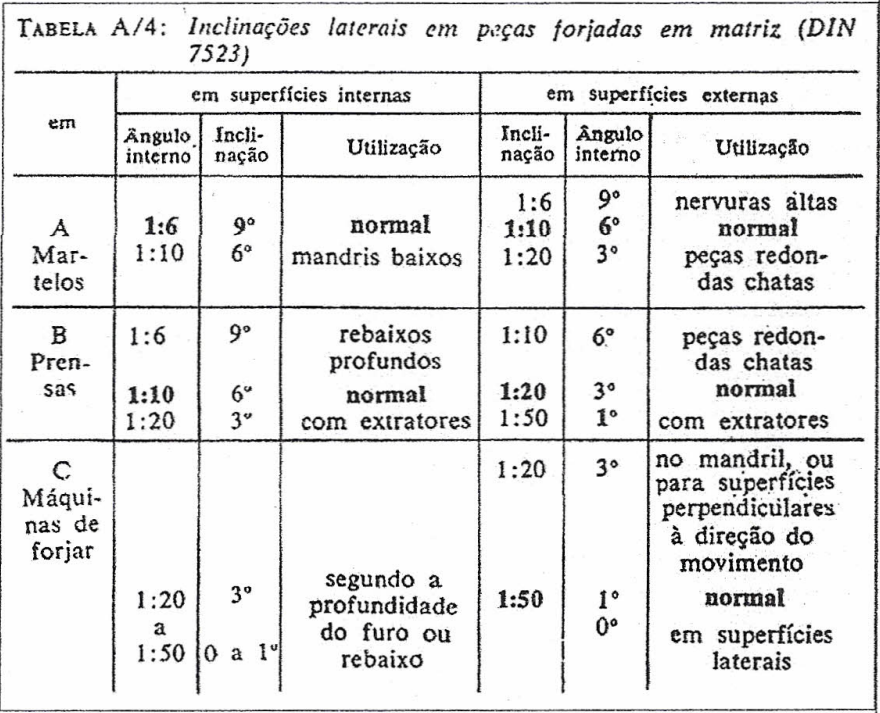
\includegraphics[width=1\linewidth]{Imagens/Tabela A4.png}
    \smallcaption{Fonte: \textcite{Formulario}}
    \label{tab:tabA4}
\end{table}

O próximo passo foi escolher através das Tabelas \ref{tab:tabA5} e \ref{tab:tabA6} os ângulos de arredondamento para o forjado.
\newpage
\begin{table}[!htb]
 \centering
    \caption{Tabela A/5}
    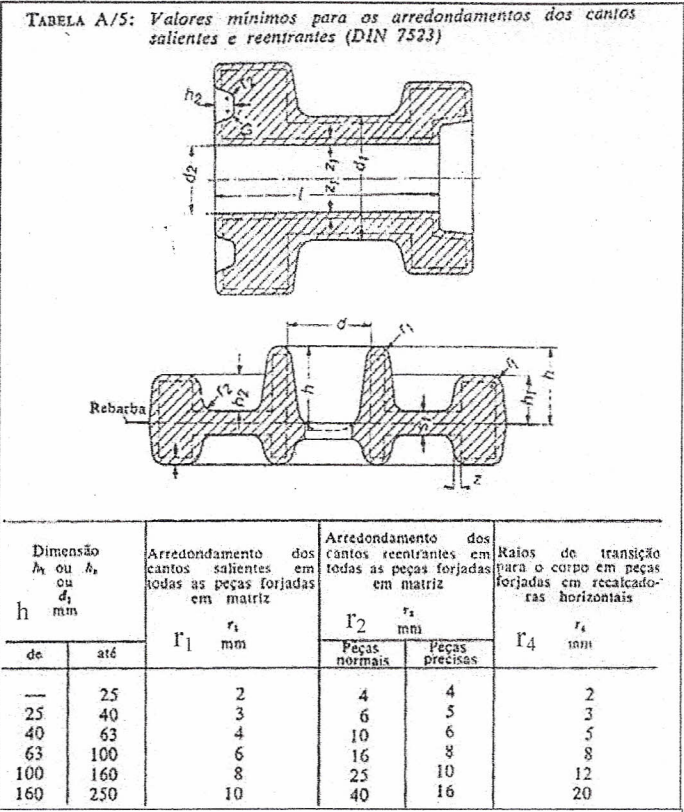
\includegraphics[width=1\linewidth]{Imagens/Tabela A5.png}
    \smallcaption{Fonte:\textcite{Formulario}}
    \label{tab:tabA5}
\end{table}

\begin{table}[!htb]
 \centering
    \caption{Tabela A/6}
    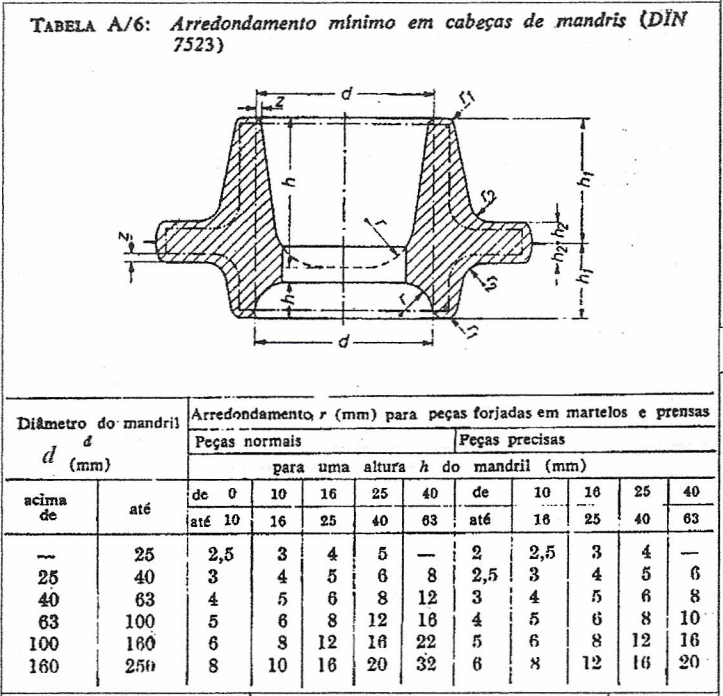
\includegraphics[width=1\linewidth]{Imagens/Tabela A6.png}
    \smallcaption{Fonte:\textcite{Formulario}}
    \label{tab:tabA6}
\end{table}


\newpage

Com os raios já devidamente escolhidos e a peça cotada foi feita a escolha das tolerâncias a partir das Tabelas \ref{tab:tab1} e \ref{tab:tab7}, para as cotas e raios, respectivamente.

\begin{table}[!htb]
 \centering
    \caption{Tabela 1}
    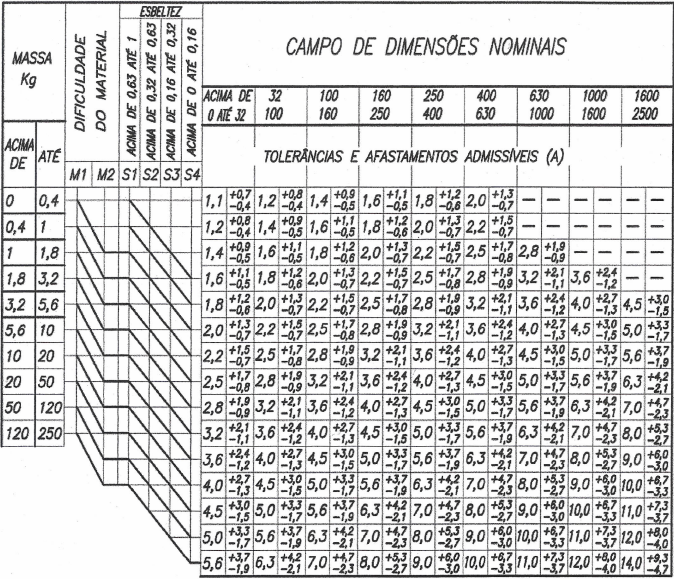
\includegraphics[width=1\linewidth]{Imagens/Tabela 1.png}
    \smallcaption{Fonte:\textcite{Formulario}}
    \label{tab:tab1}
\end{table}

\begin{table}[!htb]
 \centering
    \caption{Tabela 7}
    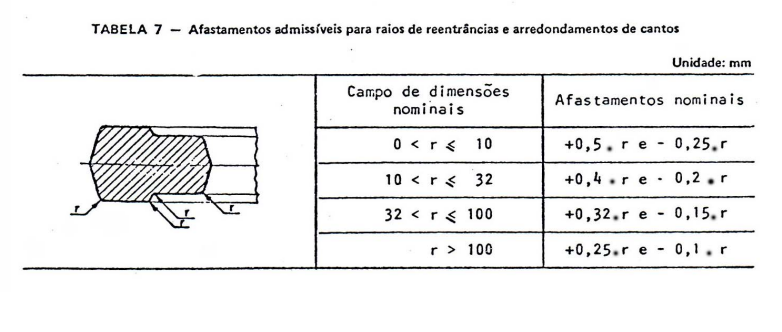
\includegraphics[width=1\linewidth]{Imagens/Tabela 7.png}
    \smallcaption{Fonte: \textcite{Formulario}}
    \label{tab:tab7}
\end{table}
\newpage
Também foi necessária a utilização da Tabela \ref{tab:tabA3} para a definição das dimensões da bacia de rebarba externa.

\begin{table}[!htb]
 \centering
    \caption{Tabela A/3 com figura A37}
    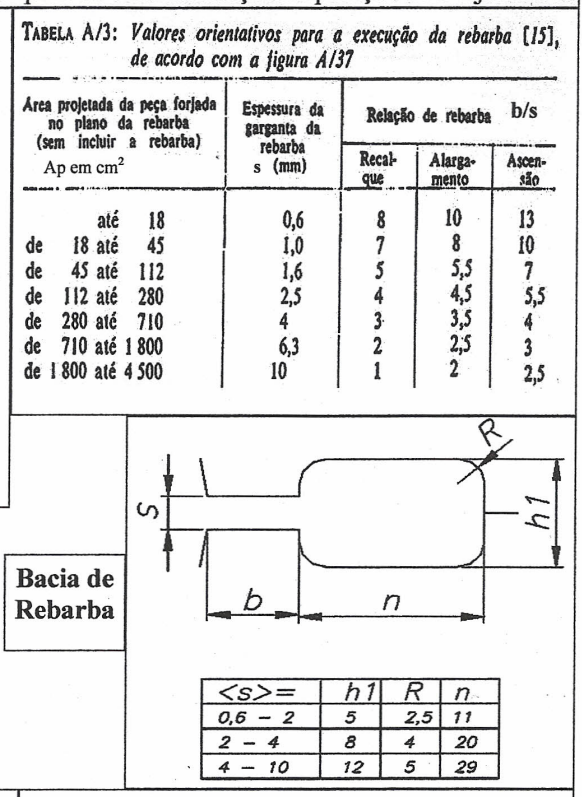
\includegraphics[width=0.8\linewidth]{Imagens/Tabela A3 fig A37.png}
    \smallcaption{Fonte: \textcite{Formulario}}
    \label{tab:tabA3}
\end{table}

Por fim, a Tabela \ref{tab:tabA2} foi utilizada para dimensionar a matriz de forjamento. 
\begin{table}[!htb]
 \centering
    \caption{Tabela A/2}
    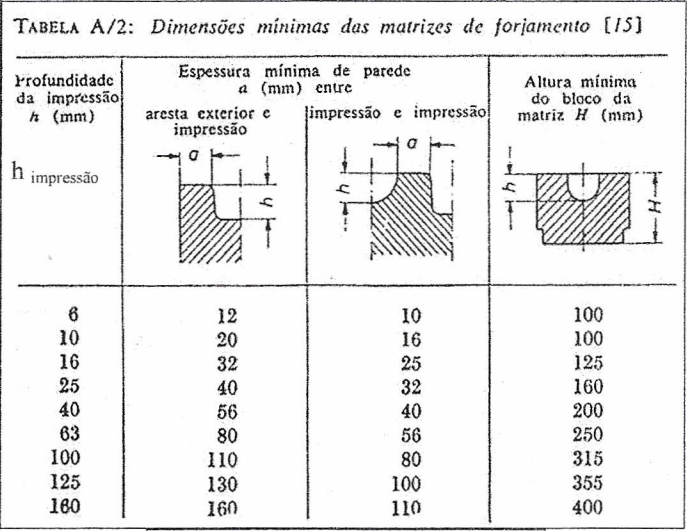
\includegraphics[width=1\linewidth]{Imagens/Tabela A2.png}
    \smallcaption{Fonte: \textcite{Formulario}}
    \label{tab:tabA2}
\end{table}


\chapter{Metodologia}


Para iniciar o projeto, primeiramente foi realizado o 2D da peça usinada no software \textit{AutoCAD} com as medidas, material da peça e temperatura de forjamento, pré-estabelecidos pelo professor. Desenhada a peça, foi possível, através de cálculos que serão explicados no capítulo \ref{resultados}, a realização do 2D da peça forjada e algumas considerações foram feitas, sendo elas: o sobremetal, a posição das linhas de rebarbas internas e externas, os raios e os ângulos de arredondamento. Seguindo em frente foi realizado os cálculos das tolerâncias do forjado através de tabelas normalizadas.

Após a realização do 2D do forjado seguiu-se para a realização do projeto das matrizes de forjamento. Para isso, foi calculado, com o auxílio do material de aula do professor e das tabelas citadas no capítulo \ref{tabelas}, o espaçamento mínimo entre as impressões e a altura mínima dos estampos. 

Com as matrizes dimensionadas o próximo passo foi dimensionar o Blank Cortado, medindo por meio do volume do Blank a altura $H$ e por meio do desenho do forjado o $D_{bitola}$, que por sua vez teve que ser normalizado para se adequar às normas. Com esse valores foi possível verificar a resistência à flambagem do projeto. 

Por fim, foi realizado o cálculo dos esforços de forjamento pelos métodos da estimativa simplificada (Grünning), diagrama simplificado (MÄKELT) e elementos finitos. No fim, foi feita uma comparação dos métodos para uma melhor análise.

Vale ressaltar que toda a metodologia será mais detalhada no próximo capítulo. E que a realização deste projeto foi todo baseado nas normas DIN EN 10254 e DIN EN 10243. 


\chapter{Resultados obtidos e discussão} \label{resultados}

%RESULTADOS EM FORMA DE TABELAS COM PASSO A PASSO DA CONSTRUÇÃO (ORIGEM DOS VALORES) NA PRÓPRIA TABELA.

%DETALHAMENTO DA SIMULAÇÃO: PRINT DE TUDO QUE FOR POSSÍVEL 

%DESENHOS NECESSÁRIOS:

%BLANK FORJADO FINAL SEM REBARBAS COM COTAS E TOLERANCIAS, MATERIAL E ETC.

%SEQÊNCIA DE FABRICAÇÃO COM AS DIMENSÕES NOMINAIS: BLANK CORTADO, BLANK FORJADO C/ REBARBAS, BLANK FINAL S/ REBARBAS E PEÇA USINADA

%MATRIZES SUPERIOR E INFERIOR COM COTAS E TOLERÂNCIAS, DUREZA E MATERIAL

%NÃO APARECEU O FOLDING MAS NÃO SE PREOCUPAR POR SER SIMULAÇÃO MAS EM CASOS REAIS RECOZER E REFAZER TODA A SIMULAÇÃO
\section{Resultados calculados}

Para que seja possível realizar as simulações da peça forjada é necessário uma peça usinada. Portanto as medidas iniciais do usinado, a temperatura e o material da peça foram dados ao grupo pelo professor e se encontram na Tabela \ref{tab:medidas} e as referências das tamanhos (A-K) se encontram na Figura \ref{fig:medidasak}.

\begin{table}[!htb]
 \centering
    \caption{Medidas fornecidas para a peça usinada}
    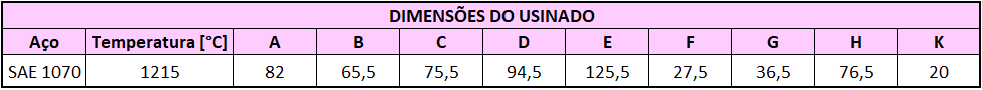
\includegraphics[width=1\linewidth]{Imagens/tabela de medidas usinado.png}
    \smallcaption{Fonte: Material de aula}
    \label{tab:medidas}
 \end{table}

\begin{figure}[!htp]
    \centering
    \caption{Dimensões da peça usinada}
    \includegraphics[width=0.6\linewidth]{Imagens/dimensões do usinado original.png}
    \smallcaption{Fonte: Material de aula}
    \label{fig:medidasak}
\end{figure}

Com estes dados em mãos possibilitou a construção, no software \textit{AutoCAD}, a peça usinada solicitada, mostrada na Figura \ref{fig:peçausinada} e posteriormente a criação do 3D, mostrada na Figura \ref{fig:peçausinada3d}. A Figura \ref{fig:peçausinadapro} mostra as propriedades da peça usinada.

\begin{figure}[!htp]
    \centering
    \caption{Dimensões do usinado com as dimensões solicitadas }
    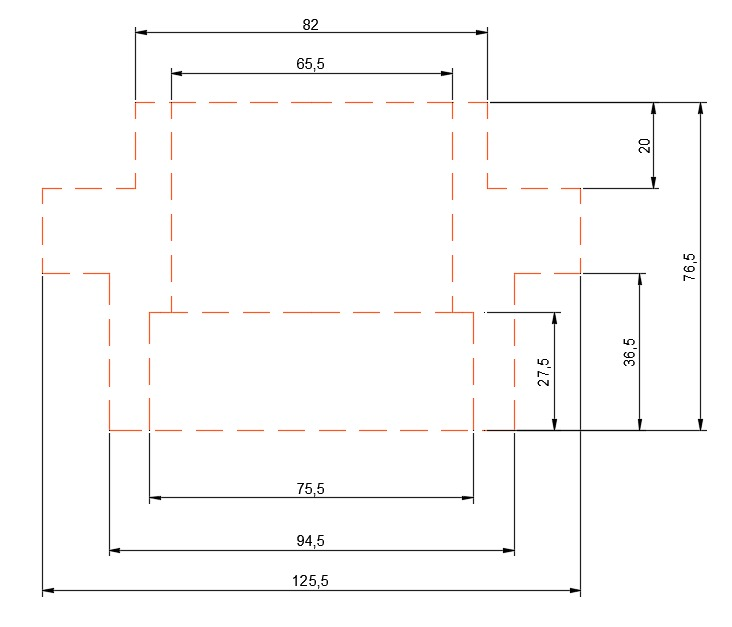
\includegraphics[width=0.7\linewidth]{Imagens/cotas usinados certo.jpeg}
    \smallcaption{Fonte: Autor}
    \label{fig:peçausinada}
\end{figure}

\begin{figure}[!htp]
    \centering
    \caption{3D do usinado}
    \includegraphics[width=0.7\linewidth]{Imagens/Peça Usinada Isometrica - Grupo 6.png}
    \smallcaption{Fonte: Autor}
    \label{fig:peçausinada3d}
\end{figure}

\newpage

\begin{figure}[!htp]
    \centering
    \caption{Propriedades do usinado}
    \includegraphics[width=0.7\linewidth]{Imagens/Peça Usinada Propriedades - Grupo 6.png}
    \smallcaption{Fonte: Autor}
    \label{fig:peçausinadapro}
\end{figure}

\newpage

Com a peça usinada desenhada foi possível realizar o desenho do forjado, mostrado na Figura \ref{fig:peçaforjada} com os tamanhos originais sem as tolerâncias que serão discutidas com mais detalhes durante o relatório. 

\begin{figure}[!htp]
    \centering
    \caption{Dimensões do forjado}
    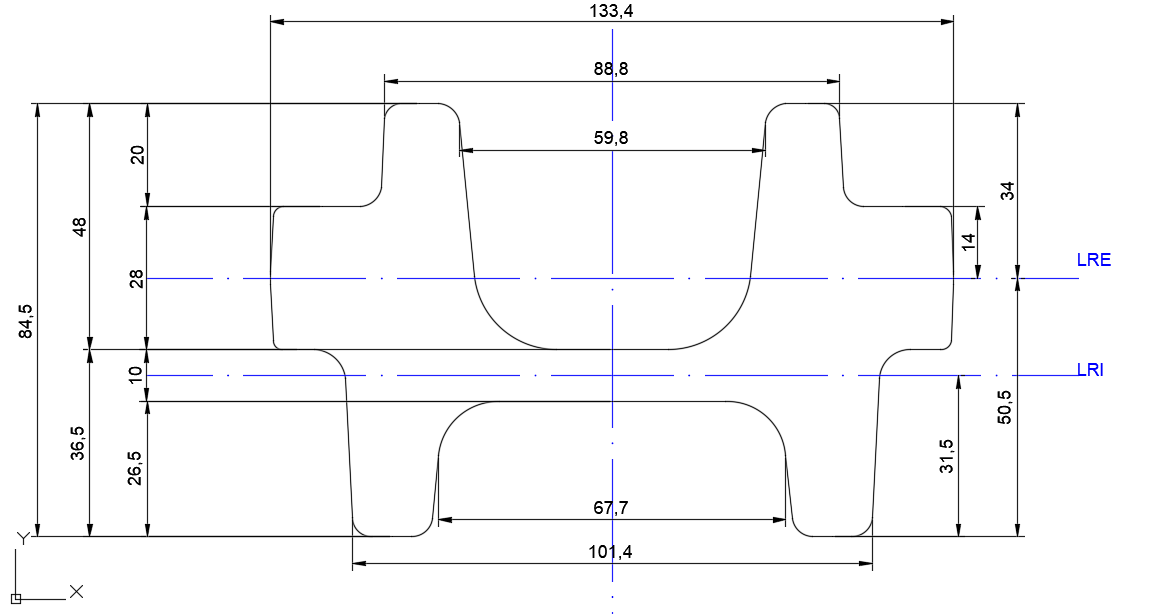
\includegraphics[width=0.8\linewidth]{Imagens/cotas forjado certo.png}
    \smallcaption{Fonte: Autor}
    \label{fig:peçaforjada}
\end{figure}

Após a realização do 2D do forjado foi feito o 3D do mesmo, mostrada na Figura \ref{fig:peçaforjadaiso}, a Figura \ref{fig:peçaforjadaprop} mostra as propriedades da peça 3D forjada que serão utilizadas mais a frente no projeto.

\begin{figure}[!htp]
    \centering
    \caption{Peça forjada}
    \includegraphics[width=0.5\linewidth]{Imagens/Peça Forjada Isometrica - Grupo 6.png}
    \smallcaption{Fonte: Autor}
    \label{fig:peçaforjadaiso}
\end{figure}


\begin{figure}[!htp]
    \centering
    \caption{Propriedades do forjado}
    \includegraphics[width=0.5\linewidth]{Imagens/Peça Forjado Propriedades - Grupo 6.png}
    \smallcaption{Fonte: Autor}
    \label{fig:peçaforjadaprop}
\end{figure}


\newpage
\subsection{Classificação do forjado}

Com os dados fornecidos e a peça usinada desenhada foi possível realizar todos os cálculos e validações para a peça forjada como o material da matriz e a força de forjamento. E assim foi possível fazer a classificação do forjado, segundo as normas DIN EN10254 e 10243. A qualidade do forjado, o grupo do material, o índice de esbeltez e o tipo de rebarba achados estão dispostos na Tabela \ref{tab:cl forj}.

\begin{table}[!htb]
 \centering
    \caption{Classificação do forjado}
    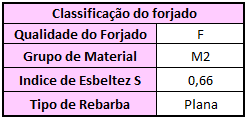
\includegraphics[width=0.4\linewidth]{Imagens/classificação .png}
    \smallcaption{Fonte: Autor}
    \label{tab:cl forj}
\end{table}

\subsubsection{Índice de esbeltez}

O cálculo do índice de esbeltez será detalhada na Fórmula \ref{eq:s}, juntamente com alguns breves apontamentos coerentes ao trabalho desenvolvido.

\begin{equation}
    \label{eq:s}
    s=\frac{m_f}{m_e}
\end{equation} 

É possível observar na Figura \ref{fig:indices} como seria um sólido envolvente cilíndrico 

\begin{figure}[!htp]
    \centering
    \caption{Sólido envolvente}
    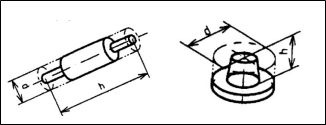
\includegraphics[width=0.5\linewidth]{Imagens/indice de esbeltez.png}
    \smallcaption{Fonte: \textcite{Formulario}}
    \label{fig:indices}
\end{figure}



O valor da massa do forjado foi retirado do modelo 3D construído, considerando as rebarbas, com isso, o valor obtido foi $m_f = 4,9 $ $kg$.

Foi calculado a massa do sólido envolvente através da Fórmula \ref{eq:me}, com um diâmetro, $d$ de $125,5mm$ e altura, $h$ de $76,5mm$, além disso a densidade assumida para o aço foi de $\rho_{aço} = 7,86\times{10^{-6}}$ $kg/mm^{3}$. O valor final foi de $7,438$ $kg$.


\begin{equation}
    \label{eq:me}
    m_e=\frac{\pi\times{d^{2}}}{4}\times{h}\times{\rho}
\end{equation} 

Após os devidos cálculos, os valores obtidos para o índice de esbeltez foi de $S = 0,66$, portanto ele pode ser classificado como $S_1$. Todos os valores encontrados estão na Tabela \ref{tab:tab inds}

 \begin{table}[!htb]
 \centering
    \caption{Índice e esbeltez}
    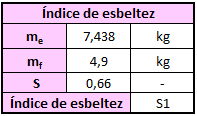
\includegraphics[width=0.3\linewidth]{Imagens/indice esbeltez.png}
    \smallcaption{Fonte: Autor}
    \label{tab:tab inds}
 \end{table}

\subsubsection{Grupo do material}
A Tabela \ref{tab:tab arce} apresenta a composição química do aço, sendo possível observar que sua porcentagem de carbono excede 65\% e, além disso, sua porcentagem dos outros elementos também ultrapassa 5\% da massa, ou seja, o aço estudado pode ser classificado como M2. 

\begin{table}[!htb]
 \centering
    \caption{Composição química do aço SAE 1070}
    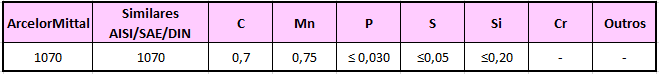
\includegraphics[width=0.8\linewidth]{Imagens/tabela arcelor.png}
    \smallcaption{Fonte: Adaptado de "Guia do Aço" ArcelorMittal}
    \label{tab:tab arce}
 \end{table}

Vale apontar que as especificações das classificações dos grupos podem ser observadas na Figura \ref{fig:M2}.

\begin{figure}[!htp]
    \centering
    \caption{Classificação quanto à qualidade}
    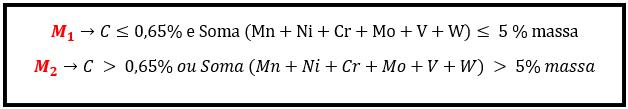
\includegraphics[width=0.6\linewidth]{Imagens/Captura de tela 2023-11-16 180524.png}
    \smallcaption{Fonte: \textcite{Classificadao}}
    \label{fig:M2}
\end{figure}

\subsubsection{Qualidade do forjado}

A respeito da qualidade do forjado, foi constatado que ele possui qualidade F, sendo comercial/normal, visto que não necessita de tolerâncias apertadas, que na maioria dos casos não seriam possíveis em processos convencionais. 

\subsubsection{Tipo de rebarba}

Ao longo do estudo, dentre os tipos de rebarba que podem ser observados na Figura \ref{fig:rebarba}, o forjado analisado foi considerado como rebarba plana, visto que sua linha de centro não sofre variações de nível.

\begin{figure}[!htp]
    \centering
    \caption{Classificação da rebarba}
    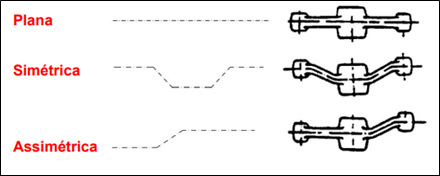
\includegraphics[width=0.6\linewidth]{Imagens/Imagem3.png}
    \smallcaption{Fonte:\textcite{Classificadao}}
    \label{fig:rebarba}
\end{figure}

\subsection{Cotas e tolerâncias}

Após a classificação do forjado é possível desenhá-lo. O desenho foi feito no software \textit{AutoCAD}, e foram adotados nomes e referências para que a identificação das cotas e tolerâncias ficasse mais fácil e menos repetitiva. As referências estão mostradas na Figura \ref{fig:refmed}.

\begin{figure}[!htp]
    \centering
    \caption{Referências adotadas para as medidas}
    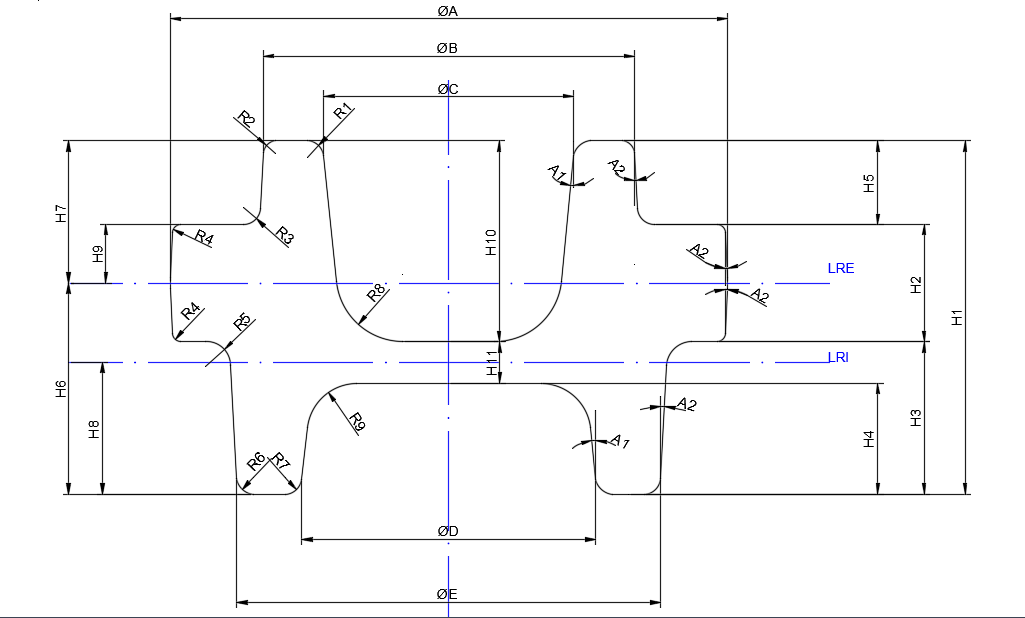
\includegraphics[width=0.8\linewidth]{Imagens/ref medidas branco.png}
    \smallcaption{Fonte: Autor}
    \label{fig:refmed}
\end{figure}

Na imagem está mostrado somente as medidas do forjado, porém são necessárias algumas medidas do usinado também, mostradas na Figura \ref{fig:peçausinada}.

\subsubsection{Ângulos de inclinação e Raios de arredondamento}

Pela imagem é possível notar que existem duas medidas $A1$ e $A2$, essas medidas são as medidas dos ângulos de saída internos e externos, respectivamente. Para calculá-los foi utilizada a norma DIN 7523 (Tabela - A/4 - Inclinações laterais em peças forjadas em matriz) e foi considerada uma prensa normal. Portanto, as inclinações internas possuem um ângulo de $6^{\circ}$ e as externas de $3^{\circ}$.

Em relação aos raios de arredondamento é necessário um pouco mais de detalhamento. Em suma, diferentemente dos ângulos de inclinação, para os raios é preciso saber também algumas outras coisas, como: 

\begin{enumerate}
    \item alturas do forjado;
    \item diâmetros do forjado e usinado;
    \item distâncias até a LRE (linha de rebarba externa);
    \item o tipo do raio.
\end{enumerate}

 
Como já dito anteriormente, é preciso saber qual o tipo de cada raio. Existem quatro tipos de raios, sendo eles: os reentrantes, os salientes, os reentrantes da cabeça do mandril e os salientes da cabeça do mandril. Para identificar os tipos de raios e achar seus valores é necessário o uso das Tabelas A/5 e A/6 normalizadas. A Tabela \ref{tab:tab dim} mostra todos os valores encontrados para os raios e os ângulos de inclinação, bem como as tabelas de onde foram tirados os dados. Vale ressaltar que as medidas indicadas na tabela são referentes as Figuras \ref{fig:peçaforjada} e \ref{fig:refmed}.

\begin{table}[!htb]
 \centering
    \caption{Dimensões dos raios e inclinações}
    \includegraphics[width=0.8\linewidth]{Imagens/tabela dimensões r e incl.png}
    \smallcaption{Fonte: Autor}
    \label{tab:tab dim}
 \end{table}

 \subsubsection{Tolerâncias}

As tolerâncias são concebidas ainda na fase de projeto para que haja uma certa segurança no momento do forjamento. Elas dependem das dimensões do material, da qualidade (F ou E), do grupo do material, da massa do forjado, e por fim, do índice de esbeltez. A Tabela \ref{tab:tab tol} mostra os resultados achado para todas as dimensões da peça, tendo como base a Figura \ref{fig:refmed} para os nomes das dimensões. A peça cotada, seguindo as normas, estará disponível nos anexos. Vale lembrar que as medidas são normalizadas e foram tiradas da Tabela 1.


\begin{table}[!htb]
 \centering
    \caption{Dimensões dos raios e inclinações}
    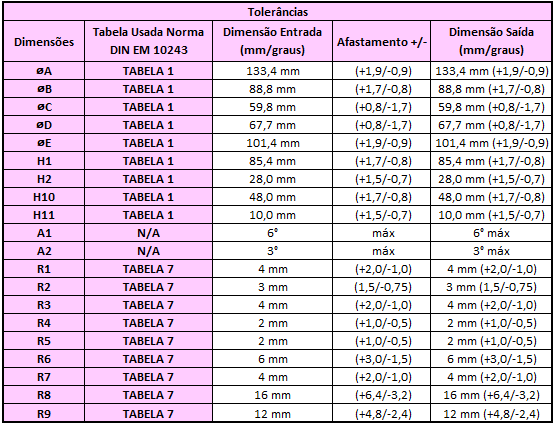
\includegraphics[width=0.8\linewidth]{Imagens/tolerancias1.png}
    \smallcaption{Fonte: Autor}
    \label{tab:tab tol}
 \end{table}
 
\newpage
\subsection{Matriz} \label{Matriz}

Para a construção da matriz foi necessário descobrir os valores do espaçamento mínimo entre as impressões ($a$) e a altura mínima dos estampos ($h$). Os valores de $h$ e $a$ são normalizados através da Tabela A/2, referenciada no capítulo \ref{tabelas}. E assim foi possível desenhar o 2D da matriz. As Figuras \ref{fig:matrizsup} e \ref{fig:matrizinf} representam as matrizes superior e inferior, respectivamente. 

\begin{figure}[!htp]
    \centering
    \caption{Matriz Superior}
    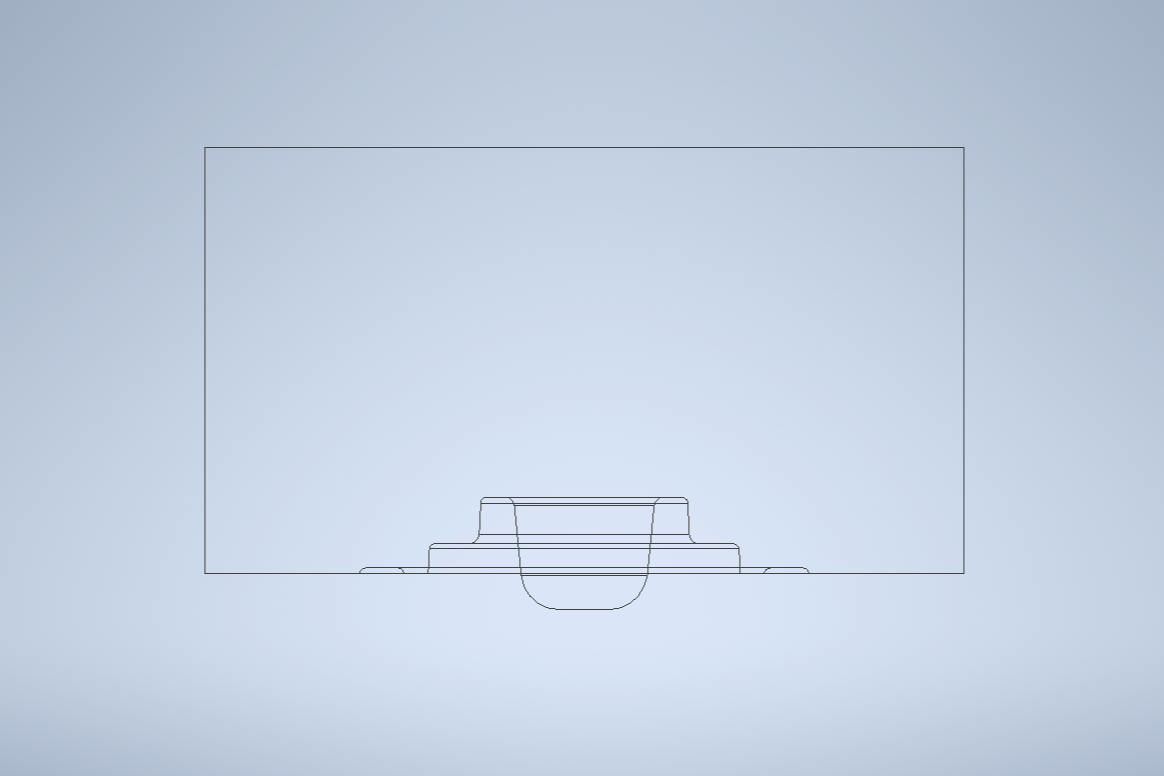
\includegraphics[width=0.6\linewidth]{Imagens/Matriz Superior - Grupo 6.png}
    \smallcaption{Fonte: Autor}
    \label{fig:matrizsup}
\end{figure}


\begin{figure}[!htp]
    \centering
    \caption{Matriz Inferior}
    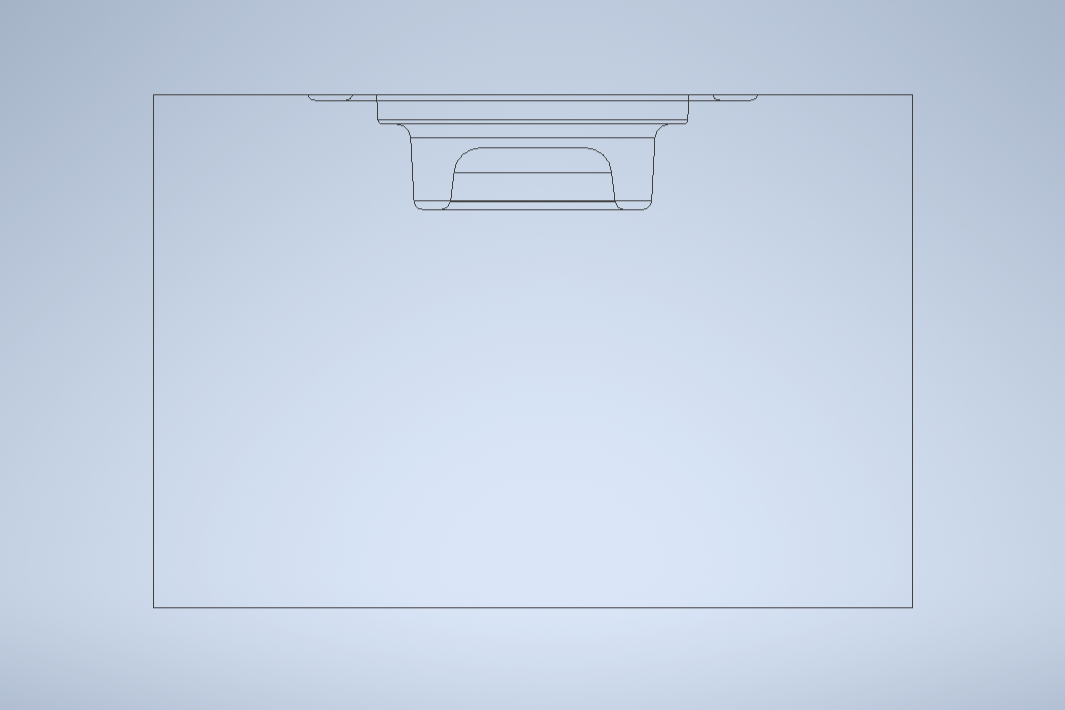
\includegraphics[width=0.6\linewidth]{Imagens/Matriz Inferior - Grupo 6.png}
    \smallcaption{Fonte: Autor}
    \label{fig:matrizinf}
\end{figure}

Os resultados achados estão na Tabela \ref{tab:tab matrizes}. Nela também estão as medidas de $h_{sup}$ e $h_{inf}$, que são as dimensões das alturas mínimas dos estampos. 

 \begin{table}[!htb]
 \centering
    \caption{Dimensões da matriz}
    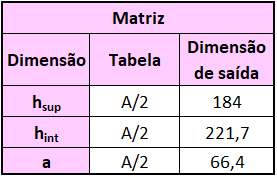
\includegraphics[width=0.3\linewidth]{Imagens/matrizes.png}
    \smallcaption{Fonte: Autor}
    \label{tab:tab matrizes}
 \end{table}
 

\subsection{Rebarba} \label{bacia}

A rebarba externa juntamente com a bacia é utilizada para que seja possível o total preenchimento da peça no momento do forjamento. Por isso é necessário que se saiba suas dimensões. A partir da Tabela A/3 normalizada isto é possível de ser realizado. A Tabela \ref{tab:tab bacia} mostra os valores achados para a dimensão da bacia de rebarba externa. 

\begin{table}[!htb]
 \centering
    \caption{Dimensões para a bacia de rebarba externa}
    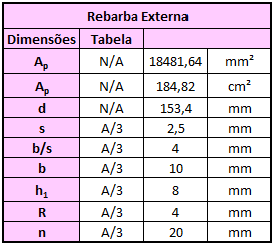
\includegraphics[width=0.4\linewidth]{Imagens/rebarba externa.png}
    \smallcaption{Fonte: Autor}
    \label{tab:tab bacia}
 \end{table}

Onde $A_p$ é a área projetada no plano da rebarba externa em $mm^{2}$ e em $cm^{2}$ e $d$ é o diâmetro projetado da rebarba, com o qual se calcula $A_p$.

Os valores de $s$, $b$, $h_1$, $R$ e $n$ são mostrados na Figura \ref{fig:dimbacia}.

\begin{figure}[!htp]
    \centering
    \caption{Bacia de rebarba externa}
    \includegraphics[width=0.3\linewidth]{Imagens/dimensão bacia1.png}
    \smallcaption{Fonte: Adaptado de norma DIN EN10254}
    \label{fig:dimbacia}
\end{figure}


\subsection{Blank Cortado}  \label{blank}

Para definir as dimensões do Blank, inicialmente foi definido o volume do forjado, sem a rebarba, que foi obtido através do software \textit{Autodesk Inventor}. E o volume da rebarba foi achado através da Equação \ref{eq:vreb}.

\begin{equation}
    \label{eq:vreb}
    V_{rebarba}= \frac{\pi\times({D^{2}-d^{2}})}{4}\times{s}
\end{equation} 

Onde $D$ é definido pela Equação \ref{eq:D}, $d$ é o diâmetro projetado da rebarba e $s$ é o mesmo da bacia da rebarba.

\begin{equation}
    \label{eq:D}
      D = d+2\times{b}
\end{equation} 

O volume total do forjado é dado pela Equação \ref{eq:vtot}. 

\begin{equation}
    \label{eq:vtot}
    V_{tot}= V_{forjado}+V_{rebarba}
\end{equation} 

A altura $H$ do Blank dever ser achada, por meio da Fórmula \ref{eq:vbl}, igualando o $V_{tot}$ e o $V_{blank}$, pois o último deve ser igual ao primeiro visto que assim se garantirá que toda a matriz fora preenchida corretamente. 

\begin{equation}
    \label{eq:vbl}
    V_{rebarba}= \frac{\pi\times({D_{bitola}^{2})}}{4}\times{H}
\end{equation} 

Onde o $D_{bitola}$ é o diâmetro $E$ na Tabela \ref{tab:tab tol} com valor de 101,4 $mm$, porém este valor não é normalizado e segundo a norma é necessário normalizá-lo para um diâmetro imediatamente menor, que no caso do projeto foi o de 95,25 $mm$.

Com os valores de $H$ e $D_{bitola}$ tem-se que testar o projeto em relação à flambagem, fazendo a relação $H/D$ e se o valor for $\leq 1,5$ o projeto é seguro. Todos os valores e resultados encontrados estão na Tabela \ref{tab:tab blank}.

\begin{table}[!htb]
 \centering
    \caption{Dimensões do Blank Cortado}
    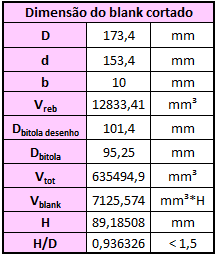
\includegraphics[width=0.3\linewidth]{Imagens/dim blank.png}
    \smallcaption{Fonte: Autor}
    \label{tab:tab blank}
 \end{table}
 
As Figuras \ref{fig:blankforj} e \ref{fig:propblankforj} mostram o blank final e suas propriedades.

\begin{figure}[!htp]
    \centering
    \caption{Blank cortado}
    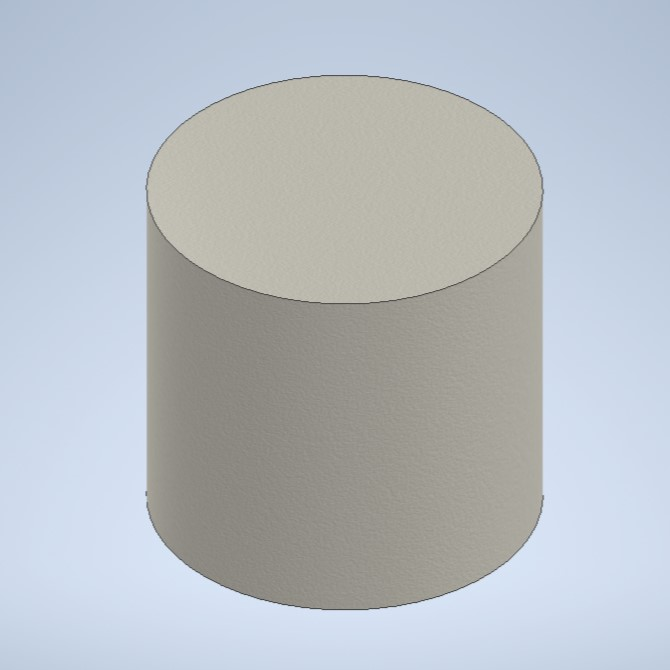
\includegraphics[width=0.3\linewidth]{Imagens/blank.jpeg}
    \smallcaption{Fonte: Autor}
    \label{fig:blankforj}
\end{figure}

 \begin{figure}[!htp]
    \centering
    \caption{Propriedades do blank cortado}
    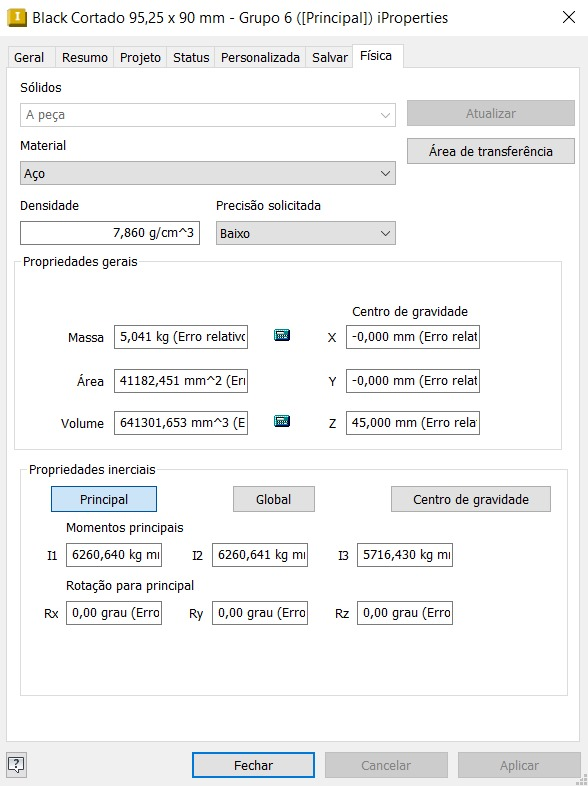
\includegraphics[width=0.4\linewidth]{Imagens/prop blank.jpeg}
    \smallcaption{Fonte: Autor}
    \label{fig:propblankforj}
\end{figure}

\newpage
\subsection{Temperatura}

Durante o projeto, foi necessário considerar a contração do material com a temperatura, ou seja, a cavidade da matriz precisa ser levemente maior que as dimensões da peça. Tendo isso em vista, foi calculado fator de concentração, que permite conhecer que percentual de aumento na matriz será necessário para comportar a contração. Os demais cálculos serão detalhados nas equações ao longo do trabalho.


Inicialmente, foi calculada a temperatura da interface forjado-matriz e a variação de temperatura [$ ^{\circ}C$], utilizando-se a temperatura do forjado e da matriz. Os cálculos podem ser visualizados nas Equações \ref{eq:Tint} e \ref{eq:deltaT}.

\begin{equation}
    \label{eq:Tint}
    {T_{INT}}= \frac{({T_{F}}+{T_{M}})}{2}=\frac{(1215+300)}{2}=757,5[^{\circ}C]
\end{equation} 

\begin{equation}
    \label{eq:deltaT}
    {\Delta_{T}}= {T_{F}}-{T_{M}}=1215-300=915[^{\circ}C]
\end{equation} 

Dando sequência, foi calculado o coeficiente de dilatação linear da interface [$ 1/^{\circ}C$], utilizando-se da temperatura da interface, como é possível observar na Equação \ref{eq:alphaint}.

\begin{equation}
    \label{eq:alphaint}
    \alpha_{INT}= (5,09091+9,09091\times{10^{-3}}\times{T_{INT}})\times{10^{-6}}=1,198\times{10^{-5}}[1/^{\circ}C]
\end{equation} 


Por fim, foi calculado o fator de contração, utilizando-se da variação de temperatura e do coeficiente de dilatação linear da interface forjado-matriz. Seu cálculo está explicado na Equação \ref{eq:FC}.

\begin{equation}
    \label{eq:FC}
    {F_{C}}= 1+\Delta_{T}\times\alpha_{INT}=1+915\times1,198\times{10^{-5}}=1,011
\end{equation} 

Com todos os cálculos efetuados, é possível observar que, para prever a contração do material, é necessário um aumento de 1,1\% da matriz em relação ao forjado. Tendo isso em vista, para a criação do modelo 3D, foi realizado um \textit{scale} de 1,011.


\subsection{Forças de forjamento} \label{Força}

A obtenção das forças de forjamento desempenha um papel crucial na indústria metalúrgica e na fabricação de peças metálicas. Essas forças são essenciais para moldar e transformar materiais brutos em produtos finais de alta qualidade e precisão.

Essas forças são de difícil obtenção, devido à diversidade de parâmetros e complexidade geométrica, sendo extremamente necessárias no pré-cálculo para oferta da peça ao cliente e no desenvolvimento do projeto em si. Nesse contexto, normalmente são estimadas por processos empíricos ou utilizando bases computacionais.

Tendo isso em vista, durante o projeto os métodos que serão utilizados para estimar as forças serão: Método da estimativa simplificada (Grünning) e  o método do diagrama de MÄKELT (Billigmann-Feldmann).

\subsubsection{Grünning} 

Para o cálculo da força de forjamento pelo método de Grünning é necessário obter a tensão média de escoamento, a área projetada da peça no plano da rebarba incluindo a rebarba e de uma constante empírica, como é possível observar na Equação \ref{eq:Fforj}.

 Dando início, foi calculada a área projetada da peça no plano da rebarba incluindo a própria rebarba, como detalhado na Equação \ref{eq:Ad}.

\begin{equation}
    \label{eq:Ad} 
    A_{d}= \frac{\pi\times({{D_{externo rebarba}}^{2})}}{4} = \frac{\pi\times({{154,8}^{2})}}{4} = 18820,5 mm^2
\end{equation} 

O valor de $\sigma_0$ foi achado através da Tabela \ref{tab:tab arce}, 

A variável C na Equação \ref{eq:Fforj} é uma constante obtida empiricamente, sendo dependente da complexidade da matriz. O valor escolhido para tal constante foi de 10, como sugerido pelo professor responsável pela disciplina.

Por fim, multiplicando os três valores calculados nas Equações \ref{eq:Ad} e EQUAÇÃO X, torna-se possível calcular a força de forjamento. Seu cálculo está detalhado na Equação \ref{eq:Fforj}. 

\begin{equation}
    \label{eq:Fforj}
    F_{Forj}= \sigma_{0}\times A_{0} \times C= \frac{39,76\times18820,5\times10}{10000}=748,2tf
\end{equation} 

\subsubsection{MÄKELT}

Para o cálculo da força de forjamento pelo método de MÄKELT é necessário obter a resistência real à deformação e a área projetada da peça no plano da rebarba incluindo a rebarba, como é possível observar na Equação \ref{eq:FforjM}. Inicialmente, foi calculada a área projetada da peça no plano da rebarba incluindo a própria rebarba. Para isso foi utilizado o diâmetro externo da rebarba, como detalhado na Equação \ref{eq:Ar}.

\begin{equation}
    \label{eq:Ar} 
    A_{r}= \frac{\pi\times({{D_{externo rebarba}}^{2})}}{4} = \frac{\pi\times({{154,8}^{2})}}{4} = 18820,5 mm^2
\end{equation} 

A fim de obter a resistência real à deformação é necessário realizar todo processo matemático especificado na Figura \ref{fig:Kr}, visto que ela é dependente de inúmeras constantes matemáticas. Estas constantes são baseadas nas seguintes variáveis: temperatura de trabalho, resistência à tração a temperatura ambiente e da relação da rebarba.

\begin{figure}[!htp]
    \centering
    \caption{Passo a passo cálculo Kr}
    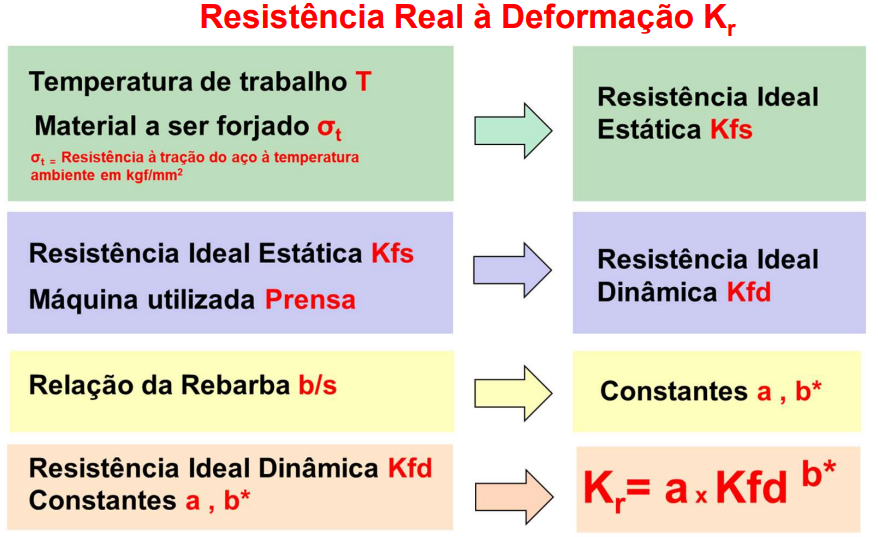
\includegraphics[width=0.6\linewidth]{Imagens/Kr.png}
    \smallcaption{Fonte: \textcite{Esfordos}}
    \label{fig:Kr}
\end{figure}

Para iniciar o cálculo, deve-se obter o valor da resistência ideal estática $Kfs$ a partir da temperatura de trabalho e do limite de escoamento do material a ser forjado. Como detalhado na Figura \ref{fig:Kfs}, deve-se pegar o intervalo em que se encontra o limite de escoamento do material para obter a fórmula correta, no caso, a Equação \ref{eq:Kfs}.

\begin{equation}
    \label{eq:Kfs}
    K_{fs}= 0,146\times 10^{14} \times T^{-4,09}=0,146\times 10^{14} \times 1215^{-4,09}=3,535 kgf/mm^2
\end{equation} 

\begin{figure}[!htp]
    \centering
    \caption{Fórmula para cálculo do Kfs}
    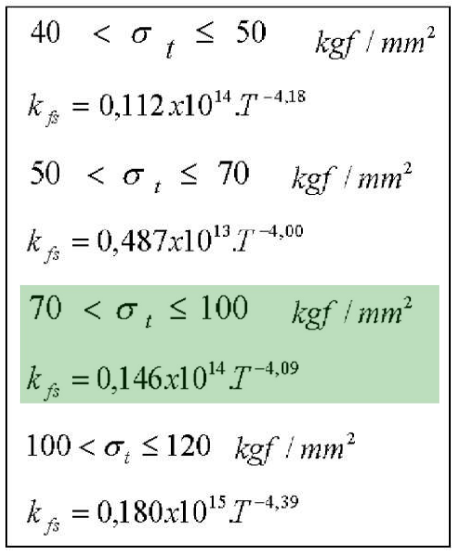
\includegraphics[width=0.3\linewidth]{Imagens/Kfs.png}
    \smallcaption{Fonte: \textcite{Formulario}}
    \label{fig:Kfs}
\end{figure}

Continuando, deve-se calcular a resistência ideal dinâmica a partir da estática. Para ser possível escolher a equação correta deve-se fornecer o equipamento utilizado, no caso, está sendo considerada a utilização de uma prensa mecânica rápida, como é visível na Figura \ref{fig:Kfd}. Com isso, a fórmula mais adequada para o caso estudado seria a detalhada na Equação \ref{eq:Kfd}.

\begin{equation}
    \label{eq:Kfd}
    K_{fd}= 3,50 \times {K_{fs}}^{0,78}=3,50 \times 3,535^{0,78}=9,372kgf/mm^2
\end{equation} 

\begin{figure}[!htp]
    \centering
    \caption{Fórmula para cálculo do Kfd}
    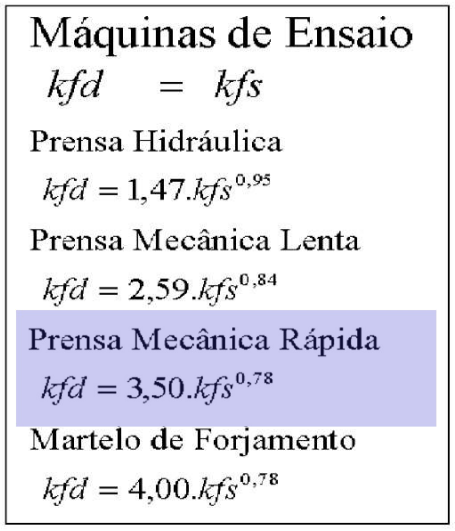
\includegraphics[width=0.3\linewidth]{Imagens/Kfd.png}
    \smallcaption{Fonte: \textcite{Formulario}}
    \label{fig:Kfd}
\end{figure}

Prosseguindo, também é necessário obter duas contantes através a utilização da relação da rebarba, que neste caso tem o valor de 4, como visto na Tabela \ref{tab:tab blank}. Neste caso, deve-se interpolar os valores das contantes $a$ e $b*$, como visto na Figura \ref{fig:ConstantesAB}. Interpolando os devidos valores, obtém-se $b*=1,037$ e $a=3,325$.

\begin{figure}[!htp]
    \centering
    \caption{Obtenção Contantes a e b*}
    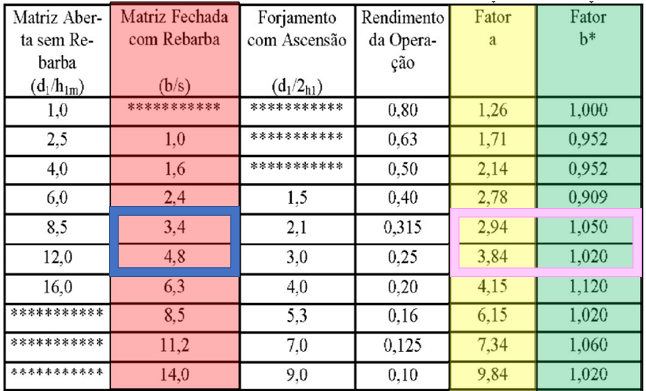
\includegraphics[width=0.6\linewidth]{Imagens/Constantes_AB.png}
    \smallcaption{Fonte: \textcite{Formulario}}
    \label{fig:ConstantesAB}
\end{figure}    

Finalmente, é possível calcular a resistência real à deformação, utilizando todas as contantes previamente calculadas, como detalhado na Equação \ref{eq:Kr}.

\begin{equation}
    \label{eq:Kr}
    K_{r}= a\times Kfd^{b*} = 3,325\times9,372^{1,037}=33,853kgf/mm^2
\end{equation} 

Em uma última análise, foi efetuado o cálculo da força de forjamento, como é possível observar na Equação \ref{eq:FforjM}. Vale citar que, ambos os valores de força de forjamento desenvolvidos no estudo foram relativamente similares, com o calculado pelo método de MÄKELT sendo um pouco mais preciso.

\begin{equation}
    \label{eq:FforjM}
    F_{Forj}= K_{r}\times A_{r} = \frac{33,853\times18820,5}{1000}=637,1tf
\end{equation} 


\section{Simulação}

Após ser obtido toda os dados e desenhos, como mostrado no capitulo foi possível iniciar as simulações para uma melhor analise da formação do Forjado e a validação das contas. 

\subsection{Geometrias}

Com a utilização do Software de desenho \textit{Autodesk Inventor} foi possível desenvolver os desenhos 3D e transportar eles para o Software \textit{Simufact Forming}, Figura \ref{fig:Geometrias}, e apos alinha-las com a linha de centro do Software, Figura \ref{fig:Alinhadas},  foi possível passar para próxima etapa. 

\begin{figure}[!htp]
  \centering
  \begin{minipage}{0.4\textwidth}
    \centering
    \caption{Todas as Geometrias no Software}
    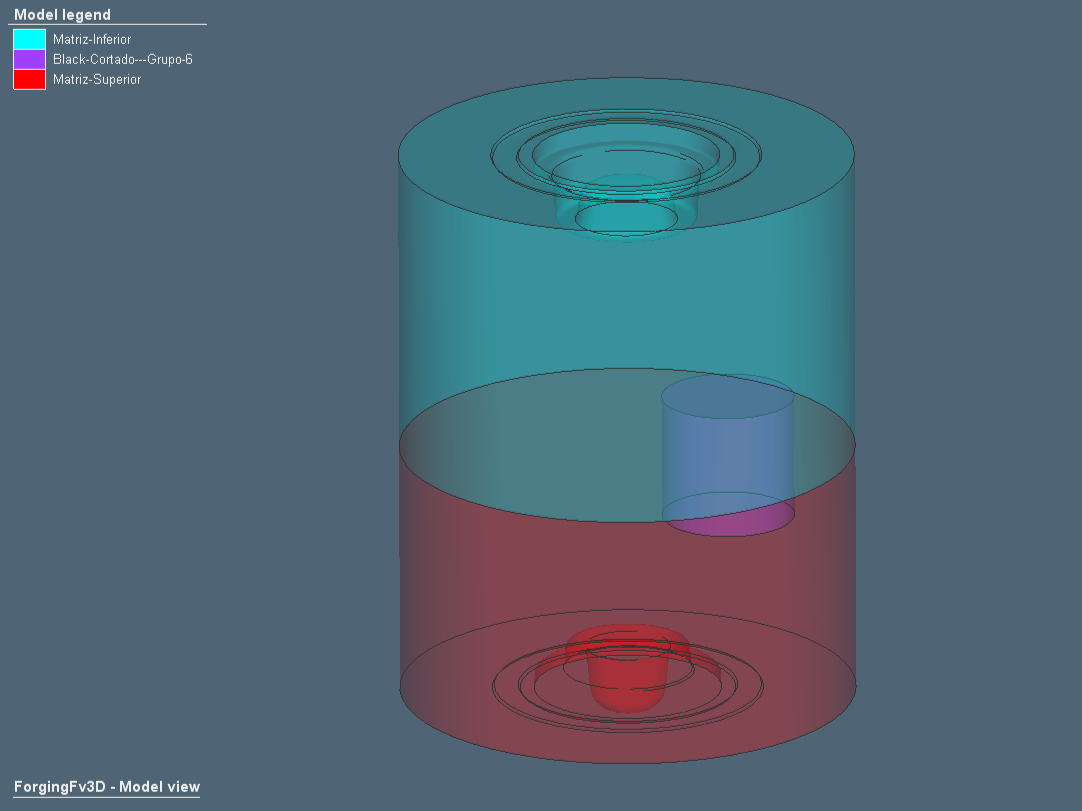
\includegraphics[width=1\linewidth]{Imagens/Simufact - Geometrias.png}
    \smallcaption{Fonte: Autor}
    \label{fig:Geometrias}
  \end{minipage}
  \hfill
  \begin{minipage}{0.4\textwidth}
        \caption{Geometrias alinhadas conforme a execução do experimento}
    \includegraphics[width=1\linewidth]{Imagens/Simufact - Peças alinhadas.png}
    \smallcaption{Fonte: Autor}
    \label{fig:Alinhadas}
  \end{minipage}
\end{figure}

\newpage

\subsection{Materiais}

O material do Blank foi definido pelo orientador, Tabela \ref{tab:medidas}, sendo o do Grupo 6 o Aço SAE 1070 que felizmente já se encontra na biblioteca do Software, Figura \ref{fig:Mforjado}, o material da Matriz foi escolhida pelo grupo na seção \ref{Matriz}, sendo esse o H-13, e este também se encontra no programa , Figura \ref{fig:Mmatriz}.

\begin{figure}[!htp]
  \centering
  \begin{minipage}{0.4\textwidth}
    \centering
    \caption{Material do Blank}
    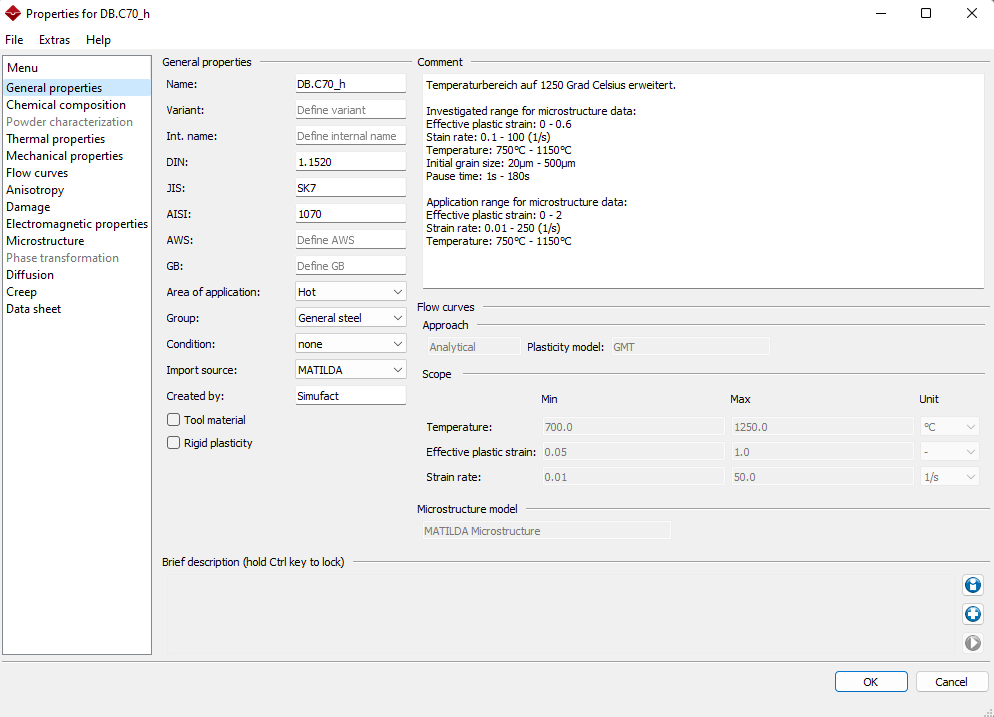
\includegraphics[width=1\linewidth]{Imagens/Simufact - Material do Forjado.png}
    \smallcaption{Fonte: Autor}
    \label{fig:Mforjado}
  \end{minipage}
  \hfill
  \begin{minipage}{0.4\textwidth}
        \caption{Material da Matriz}
    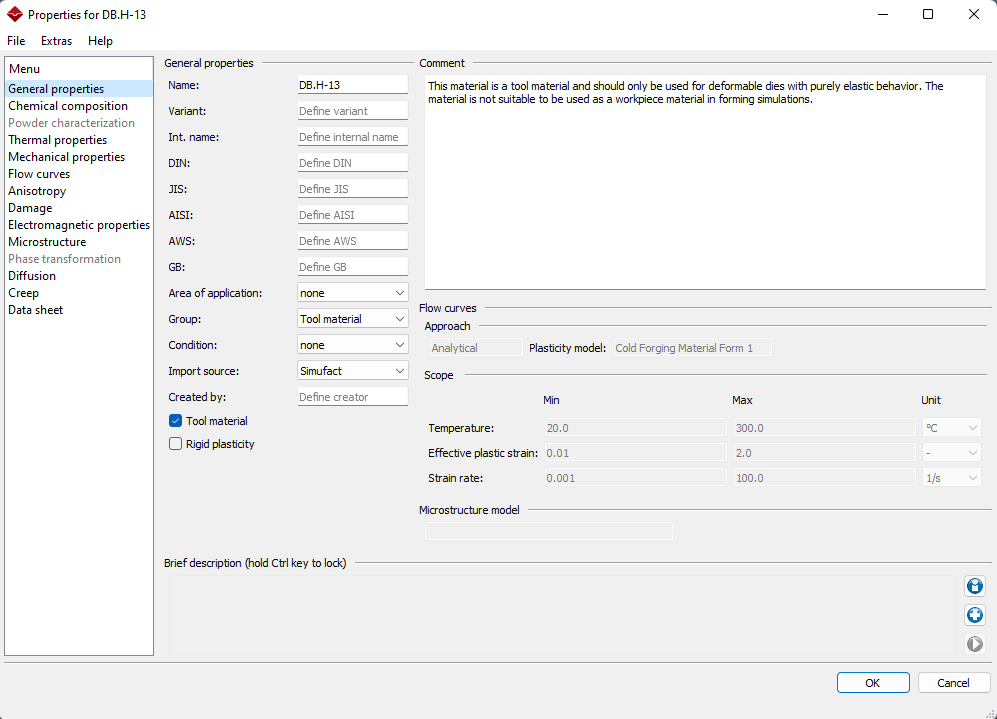
\includegraphics[width=1\linewidth]{Imagens/Simufact - Material da Matriz.png}
    \smallcaption{Fonte: Autor}
    \label{fig:Mmatriz}
  \end{minipage}
\end{figure}

\subsection{Prensas}

Como mostrado da seção \ref{Força}, entre as Forças calculadas por Grünning e Mäkelt a maior foi de Grünning com 748,22 $tonf$ na biblioteca do \textit{Simufact Forming} a preça com Força mais próxima e normalizada é DB.CP com 800 $tonf$, Figura \ref{fig:Prensa}

\begin{figure}[!htp]
    \centering
    \caption{Prensa normalizada da biblioteca do $Simufact$ $Forming$}
    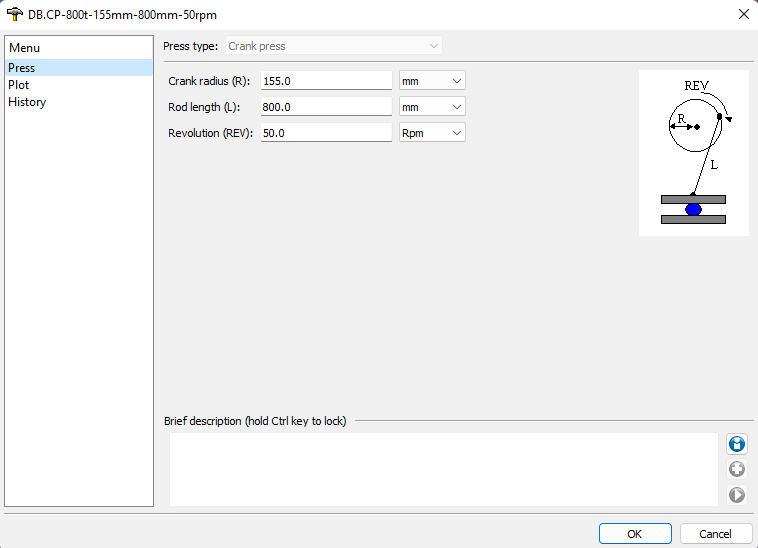
\includegraphics[width=0.7\linewidth]{Imagens/Simufact - Escolha da Ferramenta Bliblioteca.png}
    \smallcaption{Fonte: Autor}
    \label{fig:Prensa}
\end{figure}

\subsection{Fricção}

A área de estudo, que trabalho com o contato da Matriz com o Blank é muito vasta e complexa, por conta da impossibilidade de estudo de forma aprofundada no assunto utilizando-se o modelo adotado pelo professor durante as aulas, Figura \ref{fig:Fricção}.

\begin{figure}[!htp]
    \centering
    \caption{Fricção da biblioteca do $Simufact$ $Forming$ }
    \includegraphics[width=0.7\linewidth]{Imagens/Simufact - fricão .png}
    \smallcaption{Fonte: Autor}
    \label{fig:Fricção}
\end{figure}


\subsection{Calores}

Os calores adotados pelo grupo vieram através das orientações do professor, sendo a do Forjado vindo da Tabela \ref{tab:medidas} que é diferente para cada grupo, Figura \ref{fig:TBlank}.As temperaturas das Matrizes foram padrão para todos os grupos, adotando-se T = 300ºC, Figura \ref{fig:Tmatriz}.

\begin{figure}[!htp]
  \centering
  \begin{minipage}{0.4\textwidth}
    \centering
    \caption{Temperatura do Blank}
    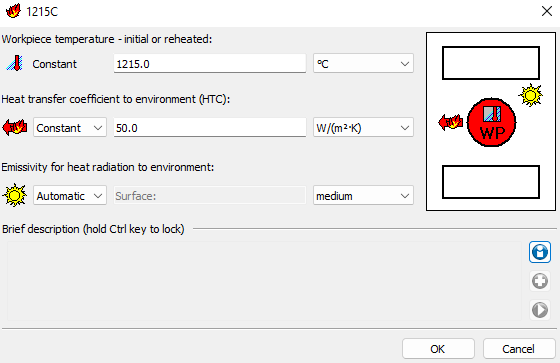
\includegraphics[width=1\linewidth]{Imagens/Simufact - Temperatura do Black.png}
    \smallcaption{Fonte: Autor}
    \label{fig:TBlank}
  \end{minipage}
  \hfill
  \begin{minipage}{0.4\textwidth}
        \caption{Temperatura da Matriz}
    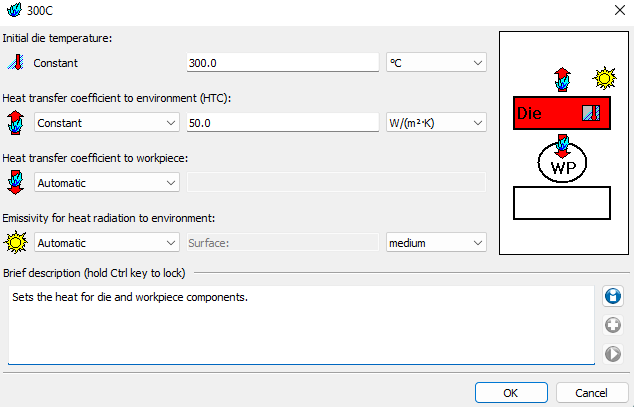
\includegraphics[width=1\linewidth]{Imagens/Simufact - Temperatura das Matrizes.png}
    \smallcaption{Fonte: Autor}
    \label{fig:Tmatriz}
  \end{minipage}
\end{figure}

\subsection{Malha} \label{malha}

Para um estudo preliminar foi escolhida a malha padrão, elaborada pelo programa, Figura \ref{fig:malha}, entretendo para posteriores Simulações haverá um melhor tratamento desta malha.

\begin{figure}[!htp]
    \centering
    \caption{Malha Padrão}
    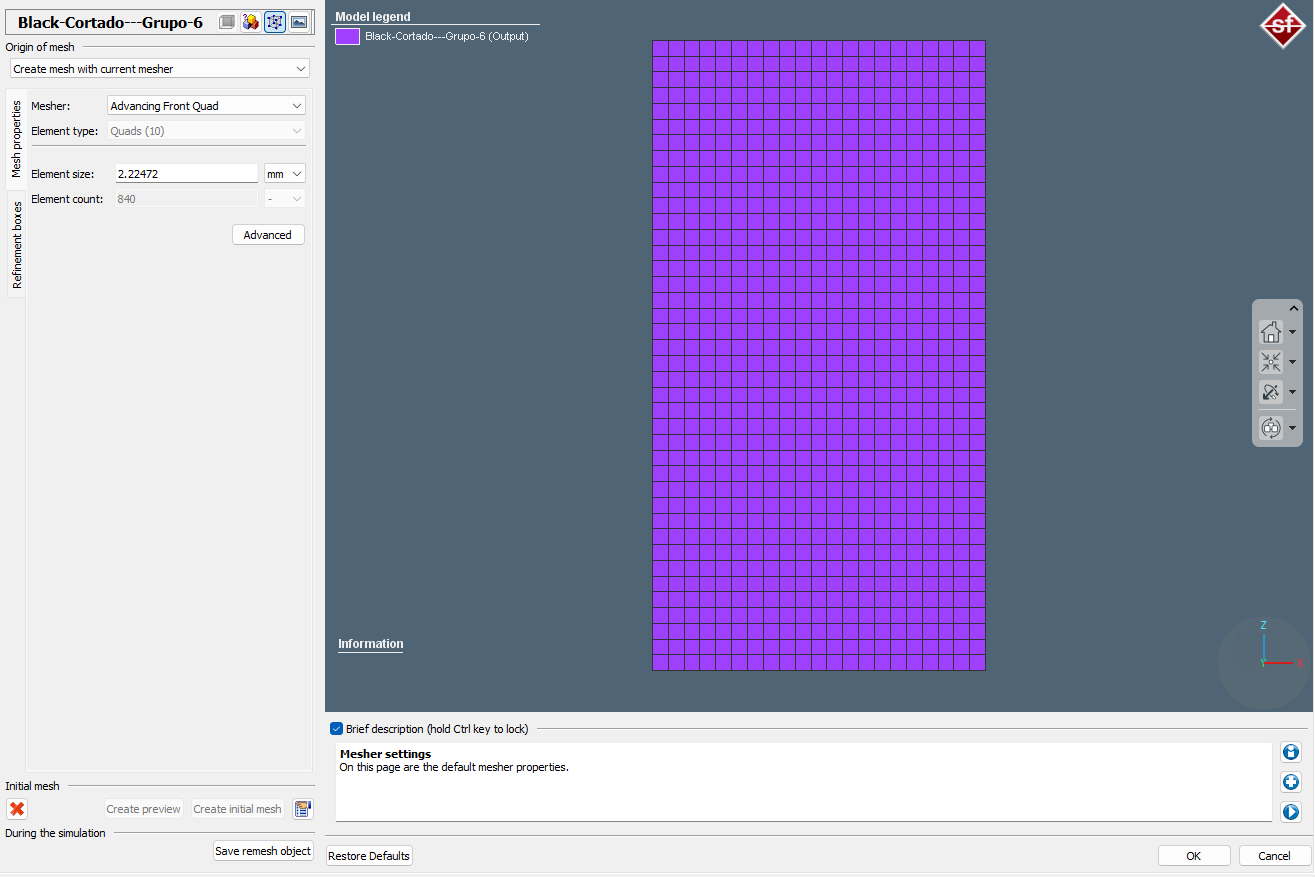
\includegraphics[width=0.7\linewidth]{Imagens/Simufact - Malha Inicial.png}
    \smallcaption{Fonte: Autor}
    \label{fig:malha}
\end{figure}


\subsection{Forming Control}

A área de Forming Control é responsável pelo movimento da Matriz para a formação do Forjado. Por se tratar de um Forjamento Vertical, seleciona-se que a Matriz Superior desça formar a distancia $s$, que neste caso será 2,5 $mm$ como mostrado da seção \ref{bacia}, com a Matriz Inferior, Figura \ref{fig:Forming}.

\begin{figure}[!htp]
    \centering
    \caption{Aba de Forming}
    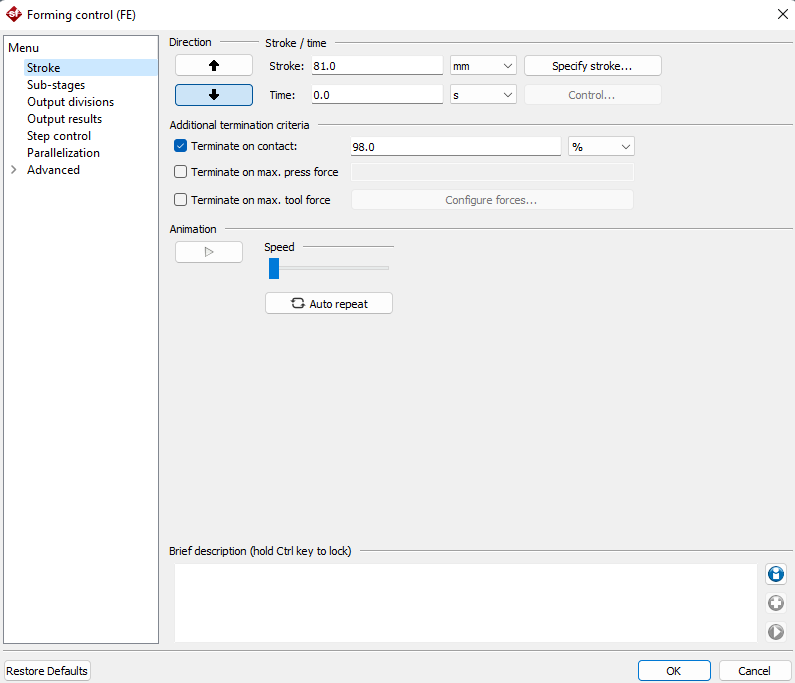
\includegraphics[width=0.7\linewidth]{Imagens/Simufact - Forming.png}
    \smallcaption{Fonte: Autor}
    \label{fig:Forming}
\end{figure}

\newpage

\subsection{Primeira Simulação}

Na execução da primeira Simulação utilizou-se o Blank Cortado de Ø95,25mm x 90mm, que foi calculado na seção \ref{blank}, utilizou-se a malha padrão da seção \ref{malha}. A tela do software antes da simulação com todos os parâmetros se encontra desta forma, Figura \ref{fig:tela}.

\begin{figure}[!htp]
    \centering
    \caption{Todos Parametros antes da Simulação}
    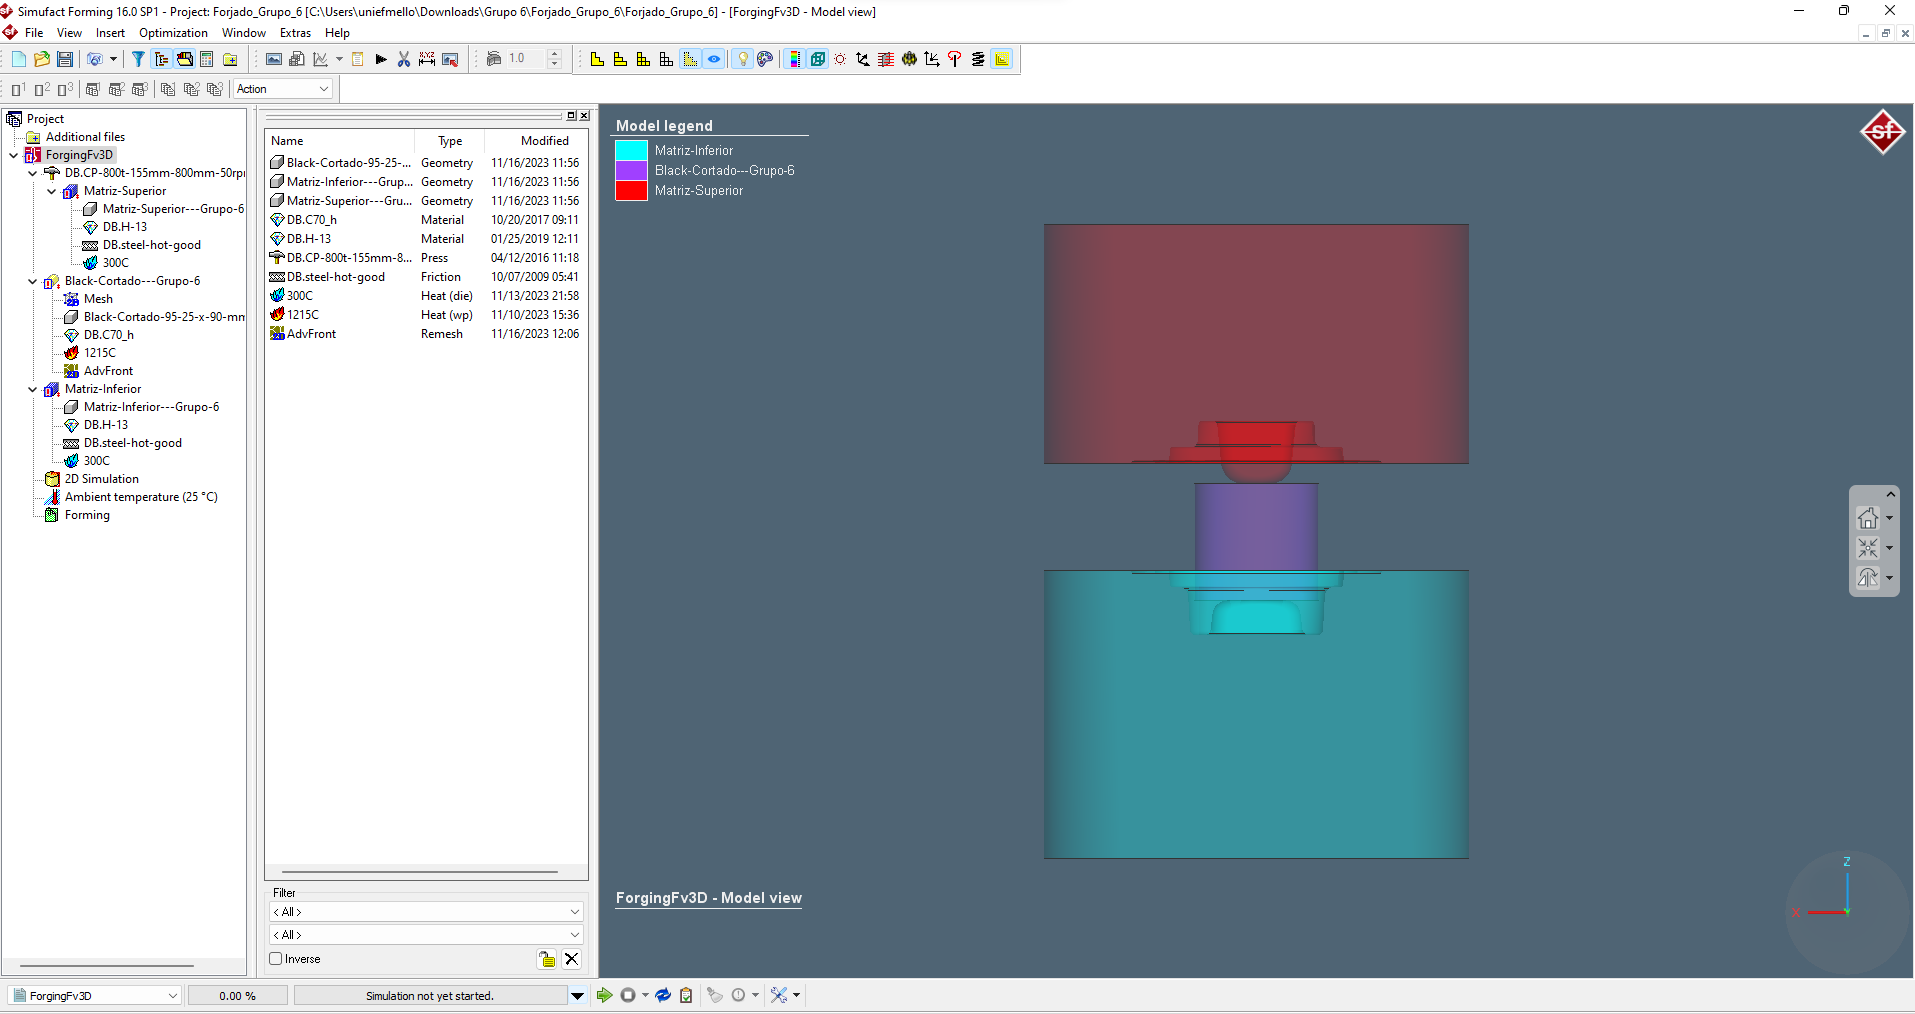
\includegraphics[width=0.7\linewidth]{Imagens/Simufact - Todos os parametros.png}
    \smallcaption{Fonte: Autor}
    \label{fig:tela}
\end{figure}

Como pode-se observar que nesta simulação preliminar, Figura \ref{fig:1simu}, não foi possível completar a rebarba da peça assim como encontra-se problema com a malha com partes de material do Blank entrando na Matriz. Outro problema que será recorrente é a ausência da areá de \textit{Fold Detection}, que foi um \textit{bug} encontrado em todos os computadores utilizados pelo grupo, e foi conversando com o professor em aula que orientou a continuar os experimentos mesmo sem a presença dessa analise, Figura \ref{fig:dobra}.

\begin{figure}[!htp]
    \centering
    \caption{Primeira Simulação}
    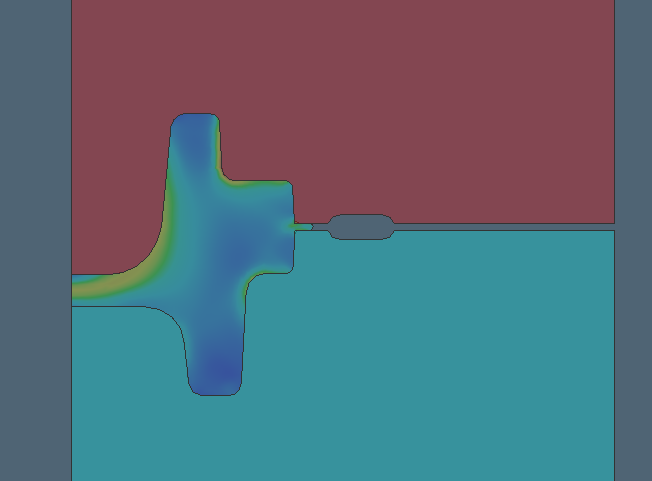
\includegraphics[width=0.7\linewidth]{Imagens/Simufact - 1º Simulação malha padrão.png}
    \smallcaption{Fonte: Autor}
    \label{fig:1simu}
\end{figure}

\begin{figure}[!htp]
    \centering
    \caption{Falta da área de Folding}
    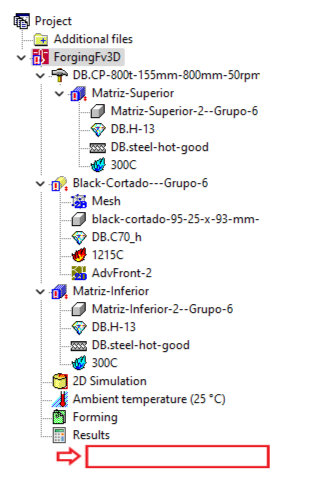
\includegraphics[width=0.3\linewidth]{Imagens/Simufact - Sem a dobra.png}
    \smallcaption{Fonte: Autor}
    \label{fig:dobra}
\end{figure}

\newpage

\subsection{Segunda Simulação}

A partir desses problemas enfrentados na primeira simulação foi decidido manter o mesmo Blank, porém utilizando uma malha mais refinada, Figura \ref{fig:malha2}. 

\begin{figure}[!htp]
    \centering
    \caption{Malha refinada}
    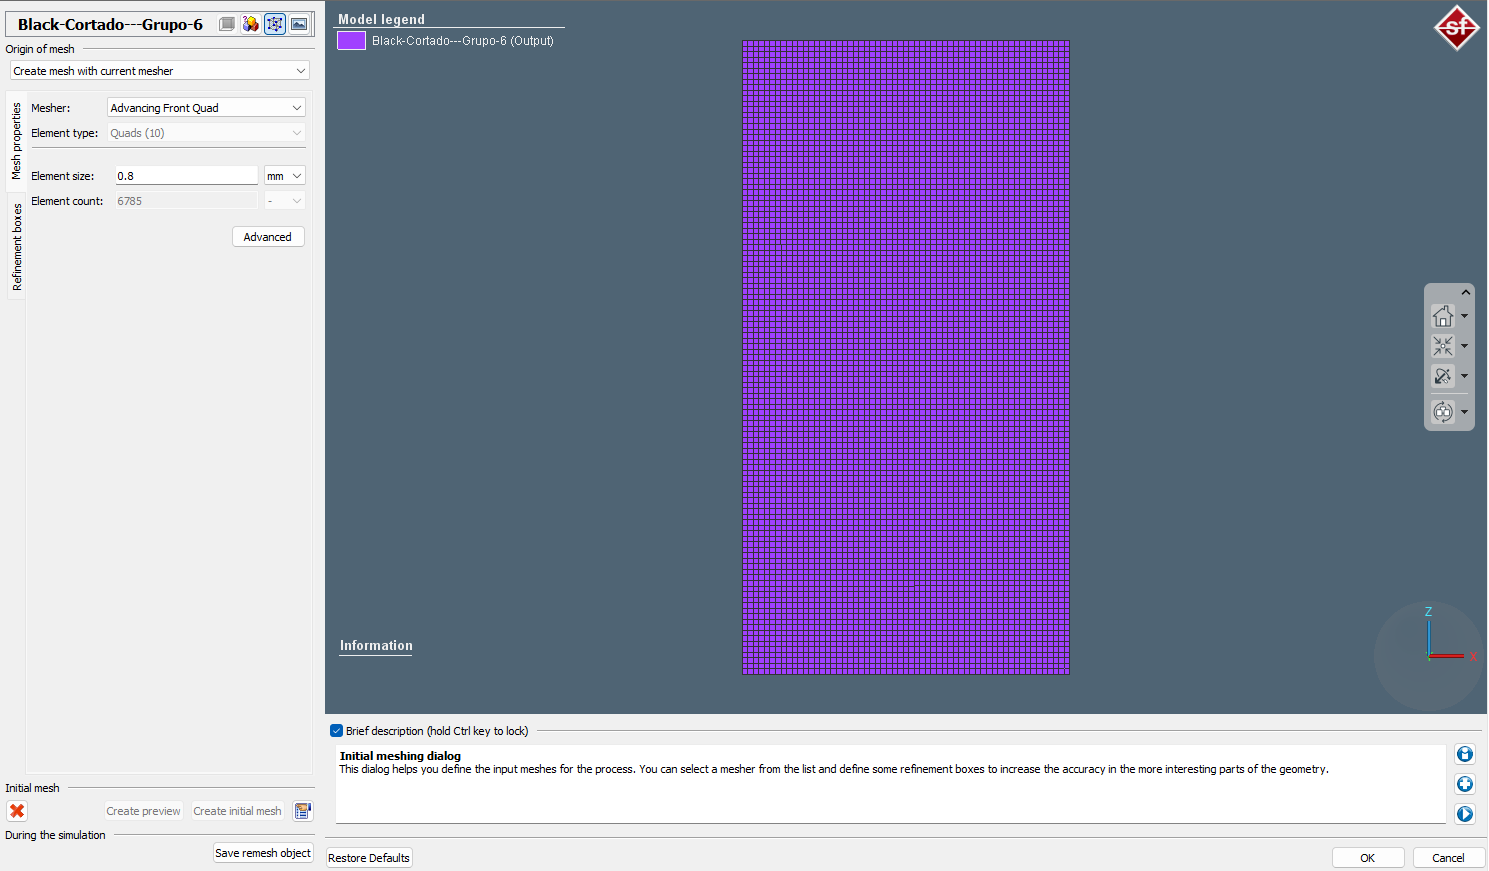
\includegraphics[width=0.7\linewidth]{Imagens/Simufact - Malha final.png}
    \smallcaption{Fonte: Autor}
    \label{fig:malha2}
\end{figure}

Ao analisar a segunda simulação, Figura \ref{fig:2simu}, percebe-se que se mantém os dois problemas anteriores, a peça não apresenta volume suficiente para completar a rebarba além do Blank continuar entrando dentro da Matriz.

\begin{figure}[!htp]
    \centering
    \caption{Segunda Simulação}
    \includegraphics[width=0.5\linewidth]{Imagens/Simufact - 2º Simulção com Zoom.png}
    \smallcaption{Fonte: Autor}
    \label{fig:2simu}
\end{figure}

\subsection{Terceira Simulação}

Para realizar a terceira simulação, utilizou-se novamente o \textit{Autodesk Inventor} e fez-se dois Raios de amortização de 2 $mm$, antes do começo do trecho da rebarba tanto da Matriz Superior quanto na Matriz Inferior, Figura \ref{fig:raios}.

\begin{figure}[!htp]
    \centering
    \caption{Matriz Superior e Inferior com os Raios de amortização}
    \includegraphics[width=0.7\linewidth]{Imagens/Raio de amortização indicado.png}
    \smallcaption{Fonte: Autor}
    \label{fig:raios}
\end{figure}

Após isso no \textit{Simufact Forming}, testou-se as novas Matriz utilizando os mesmos parâmetros da segunda simulação, Blank Cortado de Ø95,25mm x 90mm e a malha refinada. Observa-se que a o Blank não entrou mais na matriz porém continuou tendo o problema de formação da rebarba completa do Forjado, Figura \ref{fig:3simu}.

\begin{figure}[!htp]
    \centering
    \caption{Terceira Simulação}
    \includegraphics[width=0.5\linewidth]{Imagens/Simufact - 3º Simulação Matriz com raios.png}
    \smallcaption{Fonte: Autor}
    \label{fig:3simu}
\end{figure}

\subsection{Quarta Simulação}

Na quarta simulação faltava o devido preenchimento da área da rebarba, então é necessário aumentar o volume do Blank, isso pode se dar por aumento no diâmetro ou na altura, escolheu-se manter o diâmetro do Blank e aumentar a sua altura para 93,5 $mm$. Infelizmente ao fazer a simulação com esse valor, a rebarba acabou caindo para a bacia como mostrado na, Figura \ref{fig:4simu}.

\begin{figure}[!htp]
    \centering
    \caption{Quata Simulação}
    \includegraphics[width=0.5\linewidth]{Imagens/Simufact - 4º Simulação com 93,5 mm.png}
    \smallcaption{Fonte: Autor}
    \label{fig:4simu}
\end{figure}

\newpage

\subsection{Quinta Simulação}

Por fim, na quinta simulação foi selecionado o Blank Cortado com Ø95,25mm x 92,5mm, com a malha com elementos de 1,1 mm de largura e altura, Figura \ref{fig:Malha Final}.

\begin{figure}[!htp]
    \centering
    \caption{Malha Final}
    \includegraphics[width=0.7\linewidth]{Imagens/Simufact - 5Malha.png}
    \smallcaption{Fonte: Autor}
    \label{fig:Malha Final}
\end{figure}

O resultado desta simulação foi bem satisfatório como a Figura \ref{fig:Plastic} mostra. Além disso foi possível obter a rebarba completa sem nenhuma parte do material cair na bacia, Figura \ref{fig:Zoom}.

\begin{figure}[!htp]
    \centering
    \caption{Quinta Simulação}
    \includegraphics[width=0.7\linewidth]{Imagens/Simufact - 5º Plastic.png}
    \smallcaption{Fonte: Autor}
    \label{fig:Plastic}
\end{figure}

\begin{figure}[!htp]
    \centering
    \caption{Rebarba Final}
    \includegraphics[width=0.7\linewidth]{Imagens/Simufact - 5º Simulação.png}
    \smallcaption{Fonte: Autor}
    \label{fig:Zoom}
\end{figure}

\newpage

Para uma analise mais precisa da Simulação, analisou-se o contato do Blank com a Matriz, a Figura \ref{fig:Contact} mostra que houve contato total do Blank em todas as partes da Matriz, demostrando que a Simulação está coerente. Assim como é possível observar a formação completa da Geometria do Forjado com sua rebarba externa, Figura \ref{fig:5Geometria}.

\begin{figure}[!htp]
    \centering
    \caption{Contato Matriz com o Blank}
    \includegraphics[width=0.7\linewidth]{Imagens/Simufact - 5º Contact.png}
    \smallcaption{Fonte: Autor}
    \label{fig:Contact}
\end{figure}


\begin{figure}[!htp]
    \centering
    \caption{Geometria final}
    \includegraphics[width=0.7\linewidth]{Imagens/Simufact - 5Geometria.png}
    \smallcaption{Fonte: Autor}
    \label{fig:5Geometria}
\end{figure}


\newpage

\section{Comparação Teórico x Simulado}

Após realizadas as simulações, foi levantado um gráfico pelo próprio software. No Gráfico \ref{fig:grafico} é possível ver a tensão média na temperatura de forjamento. 



\begin{figure}[!htp]
    \centering
    \caption{Gráfico gerado pelo software}
    \includegraphics[width=1\linewidth]{Imagens/Simufact - Teorico x Simulação.jpg}
    \smallcaption{Fonte: Autor}
    \label{fig:grafico}
\end{figure}

Com esse dados foi possível comparar os esforços reais com os calculados. Essa comparação se encontra na Tabela \ref{tab:tab fforj}

 \begin{table}[!htb]
 \centering
    \caption{Comparação entre as forças}
    \includegraphics[width=0.4\linewidth]{Imagens/comparação fforj.png}
    \smallcaption{Fonte: Autor}
    \label{tab:tab fforj}
 \end{table}

Vale ressaltar que, para que as simulações ocorressem corretamente foi preciso manipular dados, como a altura $H$ do blank, portanto os valores distintos para a força pode ser em relação  

\chapter{Conclusões}

Apesar de terem sido elaborados todos os cálculos teóricos e seguindo corretamente o passo a passo para elaboração do forjado houveram alguns problemas pelo caminho, e os principais foram: 

1. Problema com a Matriz Original: isso se deu por conta de não ter sido adotado um chanfro ou um raio na saída da rebarba, e esse problema foi resolvido posteriormente quando fizemos novas simulações.

2. Problema com o Volume do Blank: o Blank calculado não conseguiu formar a rebarba corretamente e foi necessário aumentar o seu Volume, aumentando a altura do Blank.

3. Problema por não aparecer a Área de Dobras: este último problema ocorreu durante a simulações por um \textit{bug} do software, que não foi possível resolver.

Concluiu-se, então, que o projeto se mostrou satisfatório e cumpre com todas as normas estabelecidas. Os resultados foram favoráveis e estão dentro do esperado mesmo tendo alterações na altura $H$ do Blank Cortado em relação ao calculada, e com a alteração nas Matrizes. 

\printbibliography

\end{document}